% This is  l2kurz.tex - LaTeX2e Kurzbeschreibung v3.0
% Siehe https://github.com/texdoc/l2kurz
% arara: pdflatex: {synctex: true}
% arara: bibtex
% arara: pdflatex: {synctex: true}
% arara: pdflatex: {synctex: true}
\newcommand{\lkver}{3.0a}               % laufende Versionsnummer ...
\newcommand{\lkdate}{9.\ Juni\ 2015}   % ... und Datum

\typeout{   LaTeX2e-Kurzbeschreibung}
\typeout{   Copyright 2012,2015 Marco Daniel, Patrick Gundlach   }
\typeout{   Copyright 1998--2003 W.Schmidt, J.Knappen, H.Partl, I.Hyna   }
\typeout{   Copyright 1994, 1995 J.Knappen, H.Partl, E.Schlegl, I.Hyna   }
\typeout{   Copyright 1987 H.Partl, E.Schlegl, I.Hyna                    }

%: Start Header
\documentclass[11pt,a4paper]{article} % ergaenze `twoside', wenn gewuenscht!
%\NeedsTeXFormat{LaTeX2e}[1998/06/01]  % wegen \mathring und Textsymbolen

% Seitenlayout:
\usepackage{geometry}
 \geometry{%
  textheight=46\baselineskip,
  textwidth=5.2in,
  outer=0.5\dimexpr297mm-5.2in-2in\relax,
 }

% für die Bearbeitung ist ein großer rechter Rand von Vorteil
%\geometry{%
% textheight=46\baselineskip,
% textwidth=5.2in,
% left=1cm,
% marginpar=5cm,
%}

\usepackage[USenglish,ngerman]{babel}
\usepackage[utf8]{inputenc}
\usepackage[T1]{fontenc}
\usepackage{lmodern}
\usepackage{dtklogos}
\usepackage{textcomp,ragged2e,csquotes}
\usepackage{latexsym}
\usepackage{graphicx}
\usepackage[ngerman]{varioref}
\usepackage{array,longtable,tabularx,booktabs}
\usepackage{enumitem}

\usepackage{amsmath}

\usepackage{caption}
\makeatletter
\def\midrule{%
 \noalign{\ifnum0=`}\fi
 \penalty\@M%
  \@aboverulesep=\aboverulesep
  \global\@belowrulesep=\belowrulesep
  \global\@thisruleclass=\@ne
  \@ifnextchar[{\@BTrule}{\@BTrule[\lightrulewidth]}}

\def\arraystretch{1.5}
\makeatother

\usepackage[normalem]{ulem}

\usepackage{showexpl}
\makeatletter
\let\LTXexample\@undefined
\let\endLTXexample\@undefined
\let\LTXexample@\@undefined

\lstnewenvironment{LTXexample}[1][]
{%
  \@temptokena{#1}%
  \begingroup
    \advance\c@ltxexample\@ne \advance\c@lstlisting\@ne
    \expandafter\lstset\expandafter{\SX@explpreset,#1}%
    \edef\x{\endgroup
      \def\noexpand\SX@codefile{\SX@codefile}%
      \def\noexpand\SX@graphicname{\SX@graphicname}%
      \def\noexpand\SX@graphicparam{\SX@graphicparam}}%
  \x
  \xdef\SX@@explpreset{\the\@temptokena,codefile=\SX@codefile,
    graphic={[\SX@graphicparam]{\SX@graphicname}}}%
  \setbox\@tempboxa=\hbox\bgroup% Warum noetig?
  \def\lst@literate{}%
  \lstset{extendedchars=true,inputencoding=latin1}%
  \lst@BeginWriteFile{\SX@codefile}%
}
{%
  \lst@EndWriteFile\egroup
  \inputencoding{utf8}%
  \lstset{extendedchars=true,inputencoding=utf8}%
  \SX@put@code@result
}
\makeatother


\usepackage{wasysym}
\usepackage{xcolor}
% für todo-notes, kann später raus
\colorlet{done}{green!40}

\lstset{%
%Sprachdefinition
  language=[LaTeX]TeX,
%Definition fuer das Paket showexpl,
  pos=i,
  hsep=1cm,
  width=6cm,
  rframe={},
  explpreset={},
  numbers=none,
%Definition für listings
  basicstyle=\ttfamily\small,%
  texcsstyle=*\bfseries,
  columns=fullflexible,%
  fontadjust=true,%
  basewidth=0.65em,%
  extendedchars=true,
  inputencoding={utf8},
  upquote=true,
%Mit Farbe:
 keywordstyle=\color{blue!70!black}\bfseries,
 texcsstyle=*\color{blue!70!black}\bfseries,
 moretexcs={part,maketitle,SelectInputMappings,tableofcontents,subsection,subsubsection,chapter,mathcal,midrule,toprule,bottomrule,text,includegraphics},
% keywordsprefix={\  },
 literate=
          {\{}{\textcolor{red!70!black}{\{}}1
          {\}}{\textcolor{red!70!black}{\}}}1
          {]}{\textcolor{red!70!black}{]}}1
          {[}{\textcolor{red!70!black}{[}}1
          {Ö}{{\"O}}1
          {Ä}{{\"A}}1
          {Ü}{{\"U}}1
          {ß}{{\ss}}1
          {ü}{{\"u}}1
          {ä}{{\"a}}1
          {ö}{{\"o}}1
          {â}{{\^a}}1
          {é}{{\'e}}1
          {ð}{{\dh}}1
          {æ}{{\ae}}1
          {ô}{{\^o}}1
          {ï}{{\"\i}}1
          {ø}{{\o}}1
          {ñ}{{\~n}}1
          {♫}{{\twonotes}}1,
}

\lstnewenvironment{example}[1][]
{\lstset{xleftmargin=2cm,xrightmargin=2cm,frame=lines,belowcaptionskip=\bigskipamount,#1}}
{}


% \usepackage[textsize=footnotesize]{todonotes}

% Zum Schluss laden:
\usepackage[pdfpagelabels,pageanchor=false, linktoc=all]{hyperref}

\hypersetup{%
  pdftitle={LaTeX-Tutorium},
  pdfauthor={Tim Herbstrith},
  pdfsubject={Basierend auf Marco Daniel, Patrick Gundlach, Walter Schmidt et al.: "LaTeX2e-Kurzbeschreibung"}}




%
% Seitenzahlen oben, aber keine Kopfzeile
%
\pagestyle{myheadings}
\markboth{}{}

% Make float placement easier
\renewcommand{\textfraction}{.1}
\renewcommand{\floatpagefraction}{.7}

\makeatletter
% LaTeXe-Symbol fuer cmss/sbc mit groesserem Absstand L-a und
% halbfettem Epsilon
\DeclareRobustCommand{\sbLaTeXe}{{\fontseries{sbc}\selectfont\boldmath%
        L\kern-.25em% -.36
        {\sbox\z@ T%
         \vbox to\ht\z@{\hbox{\check@mathfonts
                              \fontsize\sf@size\z@
                              \math@fontsfalse\selectfont
                              A}%
                        \vss}%
        }%
        \kern-.15em%
        \TeX\kern.15em2$_{\textstyle\varepsilon}$}}

\makeatother
\newcommand{\cs}[1]{\texttt{\textbackslash #1}}
\newcommand\exa{\nopagebreak \begin{flushleft}\smallskip \nopagebreak
                \begin{minipage}[t]{6cm}\sloppy}
\newcommand\exb{\end{minipage}\kern 1cm\begin{minipage}[t]{8cm}\sloppy }
\newcommand\exc{\end{minipage}\kern -3cm \smallskip\end{flushleft}}

\newenvironment{beispiel}{\begin{verse}}{\end{verse}}

\newenvironment{lminipage}[1]{%
 \begin{center}\begin{minipage}{#1}\noindent\hrule\medskip}%
 {\par\noindent\hrule \end{minipage}\end{center}}

\newenvironment{ttdescription}{%
  \renewcommand{\descriptionlabel}[1]{%
    \hspace{\labelsep}\texttt{##1}}%
  \begin{description}%
}{%
  \end{description}%
}

\newcommand{\manual}{\emph{\LaTeX-Handbuch}~\cite{manual}}
\newcommand{\local}{\emph{Local Guide}~\cite{local}}

\newenvironment{symbols}{%
   \begin{tabbing}
   \hspace{1cm}\=\hspace{3.5cm}\=  \hspace{1cm}\=\hspace{3.5cm}\=
   \hspace{1cm}\=\hspace{3.5cm}\=  \kill
   }{%
   \end{tabbing}}

\newcommand{\nfrac}[2]{\leavevmode\kern.1em%
  \raise.5ex\hbox{\scriptsize #1}%
  \kern-.1em/\kern-.15em%
  \lower.25ex\hbox{\scriptsize #2}}

%: begin document
\begin{document}
\pagenumbering{Roman}
\nonfrenchspacing      % babel sets frenchspacing automatically.
%  However, some examples are pointless with frenchspacing in action.
%  Besides, the larger space after a sentence make the text more readable.
%: Einleitung
%!TEX root = l2kurz-Tutorium.tex
% Siehe https://github.com/texdoc/l2kurz

\begin{titlepage}
\renewcommand{\thefootnote}{\fnsymbol{footnote}}
{\Huge%
\fontfamily{lmss}\fontseries{sbc}\selectfont
\raggedright
\LaTeX-Tutorium
\rule{\textwidth}{0.75pt}
\par
}
\begin{flushleft}
  \normalsize
  \fontfamily{lmss}\fontseries{sbc}\selectfont
  \today\\[2ex]
  Tim B.~Herbstrith
\end{flushleft}

\vfill

{\parindent=0cm
\LaTeX{} ist ein Satzsystem, das für viele Arten von
Schriftstücken verwendet werden kann, von einfachen Briefen bis zu
kompletten Büchern.  Besonders geeignet ist es für
wissenschaftliche oder technische Dokumente. \LaTeX{} ist für
praktisch alle verbreiteten Betriebssysteme verfügbar.

Die vorliegende Kurzbeschreibung bezieht sich auf die Version
\LaTeXe\ in der Fassung vom Juni~2001 und sollte für den
Einstieg in \LaTeX{} ausreichen.
Eine vollständige Beschreibung enthält das \manual{}
in Verbindung mit der Online-Dokumentation.
}
\setcounter{footnote}{0}
\end{titlepage}


{\parindent=0cm\thispagestyle{empty}

Dieses Dokument basiert auf
\bigskip

\sbLaTeXe-Kurzbeschreibung, Version \lkver, \lkdate,\\
Copyright \copyright{} 1998--2016 M.~Daniel, P.~Gundlach, W.~Schmidt, J.~Knappen, H.~Partl, I.~Hyna veröffentlicht unter der \emph{Open Publication License}, v1.0 oder später (die aktuelle Version ist erhältlich unter
\url{http://www.opencontent.org/openpub/})
\bigskip

und wurde für das \LaTeX-Tutorium von T.~B.~Herbstrith bearbeitet und ergänzt.

Die Bearbeitung erfolgte unter Einhaltung der Lizenzbestimmungen aber \emph{ohne} individuelle Zustimmung zu den Änderungen durch die Autoren und Autorinnen des Originaldokuments.
\bigskip

% Lizenzänderung in Absprache mit Walter Schmidt <-> Patrick Gundlach 19. Juni 2012
{\selectlanguage{USenglish}
This material may be distributed only subject to the terms and
conditions set forth in the \emph{Open Publication License}, v1.0 or
later (the latest version is presently available at
\url{http://www.opencontent.org/openpub/}).}


\bigskip

Die in dieser Publikation erwähnten Software- und Hardware"=Bezeichnungen sind
in den meisten Fällen auch eingetragene Warenzeichen und unterliegen als
solche den gesetzlichen Bestimmungen.

\bigskip

\vfill

Dieses Dokument wurde mit \LaTeX{} gesetzt.
Es ist als Quelltext online erhältlich:
\begin{quote}
\url{https://github.com/tim6her/l2kurz}
\end{quote}

\bigskip

Das Originaldokument ist als Quelltext und im PDF-Format online erhältlich:
\begin{quote}
\url{http://mirror.ctan.org/info/lshort/german/}
\end{quote}
Die Änderungen gegenüber dem Originaldokument sind unter \url{https://github.com/tim6her/l2kurz/blob/master/CHANGES} einzusehen.

}


\clearpage
\pagenumbering{arabic}
\tableofcontents

\clearpage

%: Allgemeines
%!TEX root = l2kurz-Tutorium.tex
% allgemeines.tex - 1.Teil der LaTeX2e-Kurzbeschreibung v3.0
% Siehe https://github.com/texdoc/l2kurz
\section{Allgemeines}
\label{sec:allgemeines}
 
\subsection{The Name of the Game}
 
\subsubsection{\TeX}

\TeX\ (sprich "`Tech"', kann auch "`TeX"' geschrieben werden) ist
ein Computerprogamm von Donald E.~Knuth~\cite{texbook,schwarz}.
Es dient zum Setzen von Texten und mathematischen Formeln.
 
\subsubsection{\LaTeX}
 
\LaTeX\ (sprich "`Lah-tech"' oder "`Lej-tech"', kann auch
"`LaTeX"' geschrieben werden) ist ein auf \TeX\ auf\/bauendes 
Computerprogramm und wurde von Leslie Lamport~\cite{manual,wonne} 
geschrieben.  Es vereinfacht den Umgang mit \TeX, indem es 
entsprechend der logischen Struktur des Dokuments auf vorgefertigte
Layout-Elemente zurückgreift.


\LaTeXe{} ist die aktuelle Version und mit dem Fokus auf Stabilität werden derzeit nur noch Fehler behoben. Eine Weiterentwicklung findet im \LaTeX{}3"=Projekt statt, einige Zusatzmodule (\emph{Pakete}) für \LaTeX{} benutzen schon die neue Version, für den Benutzer ist dies jedoch in der Regel unsichtbar.


\subsection{Grundkonzept}
 
\subsubsection{Autor, Designer und Setzer}
 
Für eine Publikation übergab der Autor dem Verleger
traditionell  ein maschinengeschriebenes Manuskript.  Der
Buch-Designer des Verlages entschied dann über das Layout des
Schriftstücks (Länge einer Zeile, Schriftart, Abstände vor
und nach Kapiteln usw.\@) und schrieb dem Setzer die
dafür notwendigen Anweisungen dazu.
\LaTeX{} ist in diesem Sinne der Buch-Designer, 
das Programm \TeX{} ist sein Setzer.
 
Ein menschlicher Buch-Designer erkennt die Absichten des Autors
(z.\,B.\ Kapitel"=Überschriften, Zitate, Beispiele, Formeln
\dots) meistens aufgrund seines Fachwissens aus dem Inhalt des
Manuskripts.  \LaTeX{} dagegen ist "`nur"' ein Programm und
benötigt daher zusätzliche Informationen vom Autor, die die
logische Struktur des Textes beschreiben.
Diese Informationen werden in Form von sogenannten "`Befehlen"'
innerhalb des Textes angegeben.
Der Autor braucht sich also
(weitgehend) nur um die logische Struktur seines Werkes zu kümmern,
nicht um die Details von Gestaltung und Satz.
 
Im Gegensatz dazu steht der visuell orientierte Entwurf eines
Schriftstückes mit Textverarbeitungs- oder \textsc{dtp}-Programmen ("`Desktop Publishing"') wie z.\,B.\ 
\textsc{Word}.
In diesem Fall legt der Autor das Layout des Textes gleich bei der
interaktiven Eingabe fest.  Dabei sieht er am Bildschirm das, was
auch auf der gedruckten Seite stehen wird. Solche Systeme, die das
visuelle Entwerfen unterstützen, werden auch \textsc{wysiwyg}-Systeme
("`what you see is what you get"') genannt.
 
Bei \LaTeX{} sieht der Autor beim Schreiben des Eingabefiles in
der Regel noch nicht sofort, wie der Text nach dem Formatieren 
aussehen wird. Er kann aber %durch Aufruf des entsprechenden Programms 
jederzeit einen "`Probe-Ausdruck"' seines Schriftstücks auf dem
Bildschirm machen und danach sein Eingabefile entsprechend 
korrigieren und die Arbeit fortsetzen.
 
 
\subsubsection{Layout-Design}
 
Typographisches Design ist ein Handwerk, das erlernt werden muss.
Ungeübte Autoren machen dabei oft gravierende Fehler.
Fälschlicherweise glauben viele Laien, dass Textdesign
vor allem eine Frage der Ästhetik ist -- wenn das
Schriftstück vom künstlerischen Standpunkt aus "`schön"'
aussieht, dann ist es schon gut "`designed"'.
Da Schriftstücke jedoch gelesen und nicht in einem Museum
aufgehängt werden, sind die leichtere Lesbarkeit und bessere
Verständlichkeit wichtiger als das schöne Aussehen.
 
Beispiele:
Die Schriftgröße und Nummerierung von Überschriften soll so
gewählt werden, dass die Struktur der Kapitel und Unterkapitel
klar erkennbar ist.
Die Zeilenlänge soll so gewählt werden, dass anstrengende
Augenbewegungen des Lesers vermieden werden, nicht so, dass der
Text das Papier möglichst schön ausfüllt.
 
Mit interaktiven visuellen Entwurfssystemen ist es leicht,  
Schriftstücke zu erzeugen, die zwar "`gut"' aussehen,
aber ihren Inhalt und dessen Aufbau nur mangelhaft wiedergeben.
\LaTeX{} verhindert solche
Fehler, indem es den Autor dazu zwingt, die logische
Struktur des Textes anzugeben, und dann automatisch ein dafür
geeignetes Layout verwendet.

Daraus ergibt sich, dass \LaTeX{} insbesondere für  Dokumente geeignet 
ist, wo vorgegebene Gestaltungsprinzipien auf sich wiederholende
logische Textstrukturen angewandt werden sollen. 
Für das -- notwendigerweise -- visuell orientierte Gestalten
etwa eines Plakates ist \LaTeX{} hingegen 
aufgrund seiner Arbeitsweise weniger geeignet.

\subsubsection{Vor- und Nachteile}

Gegenüber anderen Textverarbeitungs- oder \textsc{dtp}-Programmen 
zeichnet sich \LaTeX{}
vor allem durch die folgenden Vorteile aus:
\begin{itemize}
\item Der Anwender muss nur wenige, leicht verständliche Befehle
  angeben, die die logische Struktur des Schriftstücks
  betreffen, und braucht sich um die gestalterischen Details
  (fast) nicht zu kümmern.
\item Das Setzen von mathematischen Formeln ist besonders gut
  unterstützt.
\item Auch anspruchsvolle Strukturen wie Fußnoten, Literaturverzeichnisse,
  Tabellen u.\,v.\,a.\  können mit wenig Aufwand erzeugt werden.
% ---- schwammige Formulierung ;-)
\item Routineaufgaben wie das Aktualisieren von Querverweisen
 oder das Erstellen des Inhaltsverzeichnisses 
 werden automatisch erledigt.
\item Es stehen zahlreiche vordefinierte Layouts zur Verfügung.
\item \LaTeX-Dokumente sind zwischen verschiedenen Installationen und
 Rechnerplattformen austauschbar.
\item Im Gegensatz zu vielen \textsc{wysiwyg}-Programmen bearbeitet \LaTeX{} auch
  lange oder komplizierte Dokumente zuverlässig,
  und sein Ressourcenverbrauch (Speicher, Rechenleistung) ist vergleichsweise
  mäßig.
\end{itemize}
Ein Nachteil soll freilich auch nicht verschwiegen werden:
\begin{itemize}
\item Dadurch, dass der Text erst von \LaTeX\ nach PDF gewandelt wird, unterscheidet sich der Arbeitsablauf von \LaTeX\ stark von den üblichen Textverarbeitungen bzw. DTP-Programmen. Das erfordert ein Umdenken und eine gewisse Einarbeitung.
\end{itemize}

\subsubsection{Der Arbeitsablauf}
Der typische Ablauf beim Arbeiten mit \LaTeX{} ist:
\begin{enumerate}
  \item Ein Eingabefile schreiben, das den Text und die \LaTeX-Befehle 
  enthält.
  \item Dieses File mit \LaTeX{} bearbeiten; dabei wird eine Datei
  erzeugt, die den gesetzten Text in einem geräteunabhängigen Format
  (\textsc{dvi}, \textsc{pdf} oder auch PostScript) enthält.
  \item Einen "`Probeausdruck"' davon auf dem Bildschirm anzeigen (Preview).
  \item Wenn nötig, die Eingabe korrigieren und zurück zu Schritt~2.
  \item Die Ausgabedatei drucken.
\end{enumerate}
Zeitgemäße Betriebssysteme machen es möglich, dass der Texteditor
und das Preview-Programm gleichzeitig in verschiedenen Fenstern 
"`geöffnet"' sind; beim Durchlaufen des obigen Zyklus brauchen sie 
also nicht immer wieder von neuem gestartet werden.  Nur die 
wiederholte \LaTeX-Bearbeitung des Textes muss noch von Hand 
angestoßen werden und läuft ebenfalls in einem eigenen Fenster ab.

Wenn der Texteditor keine Schnittstelle anbietet, um \LaTeX{} direkt aus einem Menüpunkt heraus aufzurufen, dann ist der übliche Weg über die Kommandozeile bzw. Eingabeaufforderung. Dort wird dann das Kommando \texttt{pdflatex} aufgerufen und als Parameter wird der Name der Datei angegeben, unter der das Dokument auf der Festplatte gespeichert ist.
\begin{beispiel}
  \texttt{pdflatex masterarbeit.tex}
\end{beispiel}
Das Ergebnis des Aufrufs ist eine PDF-Datei, die wie die Eingabedatei heißt, nur mit der Endung \texttt{.pdf}. \LaTeX\ gibt einige Meldungen auf der Konsole aus, die beispielsweise Auskunft über die Anzahl der Seiten des Dokuments geben.


%!TEX root = l2kurz-Tutorium.tex
% Siehe https://github.com/texdoc/l2kurz


\section{Eingabefile}

Das Eingabefile für \LaTeX{} ist ein Textfile mit der Endung \lstinline+.tex+.
Es  wird mit einem Editor erstellt und enthält sowohl den Text, der gedruckt
werden  soll, als auch die Befehle, aus denen \LaTeX\ erfährt, wie der Text
gesetzt  werden soll. Als Editor bietet sich ein spezieller \LaTeX-Editor an
wie beispielsweise Texmaker (\href{http://www.xm1math.net/texmaker}{www.xm1math.net/texmaker}). Diese Editoren bieten neben Syntaxhervorhebung
und "=überprüfung auch vordefinierte Arbeitsabläufe, so dass der Benutzer sich
auf die Erstellung des Texts konzentrieren kann. Es ist aber auch möglich und
gängige Praxis, \emph{normale} Texteditoren wie emacs, vim oder notepad++ zu
benutzen.


\subsection{Leerstellen}

"`Unsichtbare"' Zeichen wie das Leerzeichen, Tabulatoren und das Zeilenende
werden von \LaTeX{} einheitlich als Leerzeichen behandelt. \emph{Mehrere}
Leerzeichen werden wie \emph{ein} Leerzeichen behandelt. Wenn man andere als
die normalen Wort- und Zeilenabstände will, kann man dies also nicht durch die
Eingabe von zusätzlichen Leerzeichen oder Leerzeilen erreichen, sondern nur mit
entsprechenden \LaTeX-Befehlen.

Eine Leerzeile zwischen Textzeilen bedeutet das Ende eines Absatzes.
\emph{Mehrere} Leerzeilen werden wie \emph{eine} Leerzeile behandelt.


\subsection{\LaTeX-Befehle und Gruppen}

Die meisten \LaTeX-Befehle haben eines der beiden folgenden Formate: Entweder
sie beginnen mit einem Backslash~(\lstinline|\|) und haben dann einen nur aus
Buchstaben bestehenden Namen, der durch ein oder mehrere Leerzeichen oder
durch ein nachfolgendes Sonderzeichen beendet wird; oder sie bestehen aus
einem Backslash und genau einem Sonderzeichen. Groß- und Kleinbuchstaben haben
auch in Befehlsnamen \emph{verschiedene}  Bedeutung. Wenn man nach einem
Befehlsnamen eine Leerstelle erhalten will, muss  man~\lstinline|{}| zur
Beendigung des Befehlsnamens oder einen eigenen Befehl für die Leerstelle
verwenden.

\begin{LTXexample}[firstline=4]
\renewcommand*\today{%
  \the\numexpr\year-1978\relax.~Mai \the\year}
\obeylines
Heute ist der \today.
Oder: Heute ist der \today .
Falsch ist:
 Am \today regnet es.
Richtig ist:
 Am \today{} scheint die Sonne.
 Oder: Am \today\ schneit es.
\end{LTXexample}



Manche Befehle haben Parameter, die zwischen geschwungenen Klammern angegeben
werden müssen. Manche Befehle haben Parameter, die weggelassen oder zwischen
eckigen Klammern angegeben werden können. Manche Befehle haben Varianten, die
durch das Hinzufügen eines Sterns an den Befehlsnamen unterschieden werden.

Geschwungene Klammern können auch dazu verwendet werden, Gruppen (\emph{groups})
zu bilden. Die Wirkung von Befehlen, die innerhalb von Gruppen oder Umgebungen
(\emph{environments}) angegeben werden, endet immer mit dem Ende der Gruppe
bzw.\ der Umgebung.  Im obigen Beispiel ist~\lstinline|{}| eine leere Gruppe, die
außer der Beendigung des Befehlsnamens \texttt{today} keine Wirkung hat.

\subsection{Kommentare}

Alles, was hinter einem Prozentzeichen (\lstinline|%|) steht (bis zum Ende der
Eingabezeile), wird von \LaTeX{} ignoriert. Dies kann für Notizen des Autors
verwendet werden, die nicht oder noch nicht ausgedruckt werden sollen.
\begin{LTXexample}
Das ist ein % dummes
% Besser: ein lehrreiches <----
Beispiel.
\end{LTXexample}

\subsection{Aufbau}

Der erste Befehl in einem \LaTeX-Eingabefile muss der Befehl
\begin{lstlisting}
 \documentclass
\end{lstlisting}
sein. Er legt fest, welche Art von Schriftstück überhaupt erzeugt werden soll
(Bericht, Buch, Brief usw.). Danach können weitere Befehle folgen bzw.
deklariert werden, die für das gesamte Dokument gelten sollen.  Dieser Teil des
Dokuments wird auch als \emph{Vorspann} oder \emph{Präambel} bezeichnet. Mit dem
Befehl
\begin{lstlisting}
 \begin{document}
\end{lstlisting}
endet der Vorspann, und es beginnt das Setzen des Schriftstücks. Nun folgen der
Text und alle \LaTeX-Befehle, die das Ausdrucken des Schriftstücks bewirken.
Die Eingabe muss mit dem Befehl
\begin{lstlisting}
 \end{document}
\end{lstlisting}
beendet werden. Falls nach diesem Befehl noch Eingaben folgen, werden sie von
\LaTeX{} ignoriert.

Listing~\ref{mini} zeigt ein \emph{minimales} \LaTeX-File. Ein etwas
komplizierteres File ist in Listing~\ref{dokument} skizziert.

\begin{example}[caption={Ein minimales \LaTeX-File},label={mini}]
\documentclass{article}
\begin{document}
 Small is beautiful.
\end{document}
\end{example}

\begin{example}[caption={Aufbau eines Artikels},label={dokument}]
\documentclass[11pt,a4paper,ngerman]{article}
\usepackage[utf8]{inputenc}
\usepackage[T1]{fontenc}
\usepackage[ngerman]{babel}
\date{29. Februar 1998}
\author{H.~Partl}
\title{Über kurz oder lang}

\begin{document}
\maketitle
\tableofcontents

\section{Start}
Hier beginnt mein schönes Werk ...

\section{Ende}
... und hier endet es.

\end{document}
\end{example}


\subsection{Dokumentklassen}\label{docsty}

Die am Beginn des Eingabefiles  mit
\begin{lstlisting}
 \documentclass[<optionen>]{<klasse>}
\end{lstlisting}
definierte "`Klasse"' eines Dokumentes enthält Vereinbarungen über das Layout
und die logischen Strukturen, z.\,B.\ die Gliederungseinheiten (Kapitel etc.\@),
die für alle Dokumente dieses Typs gemeinsam sind.

Zwischen den geschwungenen Klammern \emph{muss} genau eine Dokumentklasse
angegeben werden.  Tabelle~\vref{docstyles} führt
Klassen auf, die in jeder vollständigen \LaTeX-Installation existieren.

Zwischen den eckigen Klammern \emph{können}, durch Kommas getrennt, eine oder
mehrere Optionen für das Klassenlayout angegeben werden. Die wichtigsten
Optionen für die Standardklassen sind in der Tabelle~\vref{options} angeführt.
Das Eingabefile für diese Beschreibung beginnt z.\,B.\ mit:
\begin{lstlisting}
 \documentclass[11pt,a4paper]{article}
\end{lstlisting}


\begin{longtable}[c]{@{}>{\raggedright\arraybackslash\ttfamily}p{2.2cm}%
                         p{\dimexpr 0.95\linewidth-2.2cm-2\tabcolsep\relax}@{}}
 \caption{Dokumentklassen}\label{docstyles} \\\toprule
\endfirsthead
 \caption[]{Dokumentklassen}\\\toprule
\endhead
 \multicolumn{2}{r}{\small Forsetzung nächste Seite}\\
\endfoot
\endlastfoot
 article &
 für Artikel in wissenschaftlichen Zeitschriften,  kürzere Berichte u.\,v.\,a.
\\
 report &
 für längere Berichte, die aus mehreren Kapiteln bestehen, Diplomarbeiten,
 Dissertationen u.\,ä.
\\
 book   &
 für Bücher
\\
 scrartcl, scrreprt, scrbook &
 Die sog. KOMA-Klassen sind Varianten der o.\,g. Klassen mit besserer Anpassung
 an DIN-Papierformate und "`europäische"' Typographie. Zudem erlauben sie
 mittels Optionen die Anpassung des Layouts. Entgegen den Standardklassen
 existiert eine deutsche und englische Dokumenation (siehe \cite{scrguide})
\\
 beamer &
 für Präsentationen
\\
\bottomrule
\end{longtable}



\begin{longtable}[c]{@{}>{\raggedright\arraybackslash\ttfamily}p{2.2cm}%
                         p{\dimexpr 0.95\linewidth-2.2cm-2\tabcolsep\relax}@{}}
 \caption[Klassenoptionen]{Klassenoptionen für die Standardklassen}\label{options} \\\toprule
\endfirsthead
 \caption[]{Klassenoptionen für die Standardklassen}\\\toprule
\endhead
 \multicolumn{2}{r}{\small Forsetzung nächste Seite}\\
\endfoot
\endlastfoot
 10pt 11pt  12pt &
 wählt die normale Schriftgröße des Dokuments aus. 10\,pt hohe Schrift ist die
 Voreinstellung; diese Beschreibung benutzt 11\,pt.
\\
 a4paper &
 für Papier im DIN\,A4-Format. Ohne diese Option nehmen die Standardklassen das
 amerikanisches Papierformat.
\\
 fleqn &
 für linksbündige statt zentrierte mathematische Gleichungen
\\
 leqno &
 für Gleichungsnummern links statt rechts von jeder   nummerierten Gleichung
\\
 titlepage  notitlepage &
 legt fest, ob Titel und Zusammenfassung auf einer eigenen Seite erscheinen
 sollen.  \texttt{titlepage} ist die Voreinstellung für die Klassen
 \texttt{report} und \texttt{book}.
\\
 onecolumn   twocolumn &
 für ein- oder zweispaltigen Satz.  Die Voreinstellung ist immer
 \texttt{onecolumn}.
\\
 oneside   twoside &
 legt fest, ob die Seiten für ein- oder zweiseitigen  Druck gestaltet werden
 sollen. \texttt{oneside} ist die Voreinstellung für alle Klassen außer
 \texttt{book}.
\\\bottomrule
\end{longtable}




\subsection{Pakete}\label{packages}

Mit dem Befehl
\begin{lstlisting}
 \usepackage[<optionen>]{<paket>}
\end{lstlisting}
können im Vorspann ergänzende Makropakete (\emph{packages}) geladen werden, die das
Layout der Dokumentklasse modifizieren oder zusätzliche Funktionalität
bereitstellen. Eine Auswahl von Paketen findet sich in der Tabelle~\vref{pack}. Der Befehl \lstinline+\usepackage+ erlaubt das Laden
mehrerer Pakete, wobei eine Optionenübergabe nicht möglich ist, bzw. die Optionen für alle Pakete gelten.



\begin{longtable}[c]{@{}>{\raggedright\arraybackslash\ttfamily}p{2.2cm}%
                         p{\dimexpr 0.95\linewidth-2.2cm-2\tabcolsep\relax}@{}}
 \caption{Pakete (eine Auswahl)}\label{pack} \\\toprule
\endfirsthead
 \caption[]{Pakete (eine Auswahl)}\\\toprule
\endhead
 \multicolumn{2}{r}{\small Fortsetzung nächste Seite}\\
\endfoot
\endlastfoot
 amsmath, amssymb &
 Mathematischer Formelsatz mit erweiterten Fähigkeiten, zusätzliche
 mathematische Schriften und Symbole; Beschreibung siehe \cite{mathmode}.
\\
 array &
 Verbesserte und erweiterte Versionen der Umgebungen  \texttt{array},
 \texttt{tabular} und \texttt{tabular*}.
\\
 babel &
 Anpassungen für viele verschiedene Sprachen. Die  gewählten Sprachen werden
 als Optionen angegeben.
\\
csquotes  & Mächtiges Paket zum korrekten Setzen (fremdsprachlicher) Anführungszeichen \\
 fontenc &
 Erlaubt die Verwendung von Schriften mit  unterschiedlicher Kodierung
 (Zeichenvorrat, Anordnung).
\\
 geometry &
 Manipulation des Seitenlayouts.\\
 graphicx &
 Einbindung von extern erzeugten Graphiken. Die umfangreichen Möglichkeiten
 dieses Pakets werden in~\cite{grfguide} und~\cite{grfcomp} beschrieben.
\\
 hyperref &
 Ermöglicht Hyperlinks zwischen Textstellen und zu externen Dokumenten;
 besonders sinnvoll einsetzbar, wenn mit \TeX\ eine Ausgabedatei im
 \textsc{pdf}- oder \textsc{html}-Format erzeugt wird.
\\
 imakeidx &
 Unterstützt das Erstellen eines Index.
\\
 listings & Flexible Erweiterung der \texttt{verbatim}-Umgebung.
\\
 longtable &
 für Tabellen über mehrere Seiten mit automatischem Seitenumbruch.
\\
microtype & Verändert den Absatzumbruch leicht, um bessere Zeilenumbrüche zu erzeugen; optischer Randausgleich. \\
 multicol &
 Mehrspaltiger Satz mit Kolumnenausgleich.
\\
 selinput &
 Deklaration der Zeichenkodierung im Eingabefile.
\\
siunitx   & Formatierung von Zahlen und physikalischen Einheiten  \\
 tabularx &
 für Tabellen mit automatisch an den vorhandenen Platz angepasster Breite der
 Spalten.
\\
 textcomp &
 Bindet Schriften mit zusätzlichen Textsymbolen ein.
 \\
 xcolor &
 Unterstützung für Farbausgabe;  Beschreibung  siehe~\cite{grfguide}
 und~\cite{grfcomp}.
\\
\bottomrule
\end{longtable}


\subsection{Eingabezeichensatz}\label{inputenc}

Bei jedem \LaTeX-System dürfen mindestens die folgenden Zeichen zur Eingabe von
Text verwendet werden:
\begin{quote}
  \ttfamily
  a\dots z A\dots Z 0\dots 9 \\
  . : ; , ? ! ` ' ( ) [ ] - / * @ + =
\end{quote}
Die folgenden Eingabezeichen haben für \LaTeX{} eine Spezialbedeutung oder sind
nur innerhalb von mathematischen Formeln erlaubt:
\begin{quote}
\verb.$ & % # _ { }  ~  ^  "  \  | < >.
\end{quote}
Für Zeichen, die über obige Liste hinausgehen, beispielsweise die Umlaute, sind
unterschiedliche Kodierungen in Gebrauch.
Die Kodierung kann in jedem (guten) Editor eingestellt werden. Es empfiehlt sich auch für englischsprachige Texte eine Kodierung zu verwenden, die zumindest lateinische Sonderzeichen zulässt.

\begin{LTXexample}
He cares a lot whether
I put a knife into
his pâté or his pate!

``maðkur'' is the
Islandic word for worm.
\end{LTXexample}


Als De-facto-Standard für die Zeichenpostion in der Kodierungstabelle hat sich der \emph{Unicode}-Standard etabliert. Für den Zugriff auf die Zeichenpostionen mittels Bit-Folgen werden \emph{Unicode Transformation Formats} (UTF) festgelegt. Am weitesten in den Anwendungen verbreitet ist \emph{UTF-8}; Betriebssysteme und Softwareentwicklungs-Frameworks verwenden häufig intern \emph{UTF-16}. Um die Eingabekodierung festzulegen, wird das Paket \texttt{inputenc} verwendet.

\begin{beispiel}
\lstinline+\usepackage[utf8]{inputenc}+
\end{beispiel}

Um ein eingegebenes Zeichen im Ausgabedokument darstellen zu können, sind noch zwei weitere Voraussetzungen notwendig. Zum einen muss die Schriftart (Font) das gewünschte Zeichen enthalten, zum anderen muss festgelegt werden, welche Bit-Folge welchem Zeichen in der Font-Kodierungstabelle entspricht.

\begin{beispiel}
\lstinline+\usepackage[T1]{fontenc}+
\end{beispiel}

Ein vollständiges Beispiel zeigt Listing~\ref{enc}.

\begin{example}[caption={Festlegen von Font- und Eingabekodierung sowie des Fonts},label={enc}]
\usepackage[T1]{fontenc}
\usepackage[utf8]{inputenc}
\usepackage{lmodern} % Latin-Modern Font Family
\end{example}

Neben dem Paket \texttt{inputenc} existiert auch das Paket \texttt{selinput}, das die Kodierung beim Kompiliervorgang ermittelt. Allerdings muss für jedes Sonderzeichen in der Präambel eine \LaTeX-Umschreibung festgelegt werden.

Falls \LaTeX{} ein eingegebenes Zeichen nicht darstellen kann, was meist für die
sogenannten "`Pseudografik-Zeichen"' gilt,  bekommt man eine entsprechende
Fehlermeldung. Auch sind manche Zeichen nur im Text, andere nur in
mathematischen Formeln erlaubt.

Man beachte, dass der in der \emph{Ausgabe} darstellbare Zeichenvorrat von
\LaTeX{} nicht davon abhängt, welche Zeichen als \emph{Eingabe} erlaubt sind:
Für jedes überhaupt darstellbare Zeichen -- also auch diejenigen, die nicht im
Zeichensatz des jeweiligen Betriebssystems enthalten sind -- gibt es einen
\LaTeX-Befehl oder eine Ersatzdarstellung, die ausschließlich mit ASCII-Zeichen
auskommt.  Näheres darüber erfahren Sie in Abschnitt \ref{spezial}.

\endinput

\clearpage
%: Textsatz
%!TEX root = l2kurz-Tutorium.tex
% Siehe https://github.com/texdoc/l2kurz

\section{Setzen von Text}


\subsection{Deutschsprachige Texte}\label{deutsch}
\LaTeX{} wurde ursprünglich für den englischen Sprachraum entwickelt.
Für Texte, die in einer anderen Sprache als (amerikanischem)
Englisch verfasst sind, muss deshalb ein zusätzliches Paket
(siehe Abschnitt~\ref{packages}) zur Sprachanpassung geladen werden.
Für deutschsprachige Texte ist das normalerweise das Paket \texttt{babel}
\begin{lstlisting}
 \usepackage[ngerman]{babel}
\end{lstlisting}
oder mit der Option \texttt{german} für traditionelle Rechtschreibung.
Der Grund für diese Unterscheidung ist die unterschiedliche Silbentrennung.
Eine ausführliche Beschreibung dieses Pakets findet man in \cite{babel}.



\subsection{Zeilen- und Seiten-Umbruch}

\subsubsection{Blocksatz}

\LaTeX{} setzt Text standardmäßig im Blocksatz, d.\,h.~mit Randausgleich,
wobei der Zeilen- und Seitenumbruch automatisch durchgeführt wird.
Dabei wird für jeden Absatz die
bestmögliche Aufteilung der Wörter auf die Zeilen bestimmt,
und wenn notwendig werden Wörter automatisch abgeteilt.
\begin{LTXexample}
Das Ende von Wörtern und
Sätzen wird durch Leerzeichen
gekennzeichnet.
Hierbei spielt es keine Rolle,
ob man ein  oder           100
Leerzeichen eingibt.

Eine oder mehrere Leerzeilen
kennzeichnen das Ende von
Absätzen.
\end{LTXexample}

Üblicherweise werden in \LaTeX{} Absätze mit Einrückungen gekennzeichnet.
Bei den Standardklassen kann dies mittels des Paketes \texttt{parskip}
deaktiviert werden und Absätze mit Abstand dazwischen kenntlich machen.
Die sogenannten KOMA-Klassen bieten hierfür extra Optionen (siehe \cite{scrguide}).

Mit Hilfe der in Abschnitt~\ref{env} beschriebenen Umgebungen ist
es möglich, spezielle Textteile jeweils anders zu setzen.

Für Ausnahmefälle kann man den Umbruch außerdem mit den
folgenden Befehlen beeinflussen:
Der Befehl \lstinline|\\| oder \lstinline|\newline| bewirkt einen
Zeilenwechsel ohne neuen Absatz, der Befehl~\lstinline|\\*| einen
Zeilenwechsel, bei dem kein Seitenwechsel erfolgen darf.
Der Befehl \lstinline|\newpage| bewirkt einen Seitenwechsel.
Mit den Befehlen
\lstinline|\linebreak[|\textit{n}\lstinline|]|,
\lstinline|\nolinebreak[|\textit{n}\lstinline|]|,
\lstinline|\pagebreak[|\textit{n}\lstinline|]|   und
\lstinline|\nopagebreak[|\textit{n}\lstinline|]|
kann man angeben, ob an bestimmten Stellen ein Zeilen- bzw.\ %
Seitenwechsel eher günstig oder eher ungünstig ist, wobei
\textit{n} die Stärke der Beeinflussung angibt (1, 2, 3 oder 4).

Mit dem \LaTeX-Befehl \lstinline:\enlargethispage{:\textit{Länge}\lstinline:}:
lässt sich eine gegebene Seite um einen festen Betrag
verlängern oder verkürzen. Damit ist es möglich, noch
eine Zeile mehr auf eine Seite zu bekommen.
(Zur Schreibweise von Längenangaben siehe Abschnitt~\ref{abst:horiz}.)

%PG: microtype erwähnt

\LaTeX\ bemüht sich, den Zeilenumbruch besonders schön zu machen.  Falls es
keine den strengen Regeln genügende Möglichkeit für einen glatten rechten Rand
findet, lässt es eine Zeile zu lang und gibt eine entsprechende Warnmeldung
aus (\texttt{over\-full hbox}). Das tritt insbesondere dann auf, wenn keine
geeignete Stelle für die Silbentrennung gefunden wird. Innerhalb der
\texttt{sloppypar}-Umgebung ist \LaTeX\ generell weniger streng in seinen
Ansprüchen und vermeidet solche überlange Zeilen, indem es die Wortabstände
stärker -- notfalls auch unschön~-- vergrößert. In diesem Fall werden zwar
Warnungen gemeldet (\texttt{under\-full hbox}), das Ergebnis ist aber meistens
durchaus brauchbar. Eine weitere Möglichkeit um \textit{schönere}  Absätze zu
erzeugen ist das Paket \texttt{microtype} für PDF\TeX{} und neuere Programme.
Es verändert einerseits die Breite der Buchstaben in einem so geringen Maß,
dass das dem Leser nicht auf"|fällt. Weiterhin erlaubt es gewisse Zeichen
etwas über den rechten Rand hinaus zu ragen (Trennstrich, Punkt, Komma,
\dots), so dass \LaTeX{} bessere Umbruchpunkte findet.



\subsubsection{Silbentrennung} \label{silb}

Falls die automatische Silbentrennung in einzelnen Fällen nicht
das richtige Ergebnis liefert, kann man diese Ausnahmen mit den
folgenden Befehlen richtigstellen.

Der Befehl \lstinline|\hyphenation| bewirkt, dass die darin
angeführten Wörter jedes Mal an den und nur an den mit
\lstinline|-| markierten Stellen abgeteilt werden können.
Er sollte im Vorspann stehen und eignet sich
\emph{nur} für Wörter, die keine indirekt kodierten Umlaute wie \lstinline|"a| enthalten.

\begin{example}
\hyphenation{ Eingabe-file
   Eingabe-files FORTRAN }
\end{example}

Der Befehl~\lstinline|\-| innerhalb eines Wortes bewirkt, dass dieses Wort
dieses eine Mal nur an den mit~\lstinline|\-| markierten Stellen  oder
unmittelbar nach einem Bindestrich abgeteilt werden kann. Mit dem Paket
\texttt{babel}\cite{babel} steht der Befehl~\lstinline:"-: zur
Verfügung, der auch Trennungen an anderen (nicht markierten) Stellen im Wort
erlaubt.

\begin{LTXexample}
Ein"-gabe"-file,
\LaTeX"=Eingabe"-file,
Häss"-lich"-keit
\end{LTXexample}

Der Befehl \lstinline|\mbox| bewirkt, dass das Argument überhaupt nicht
abgeteilt werden kann.

\begin{LTXexample}
Die Telefonnummer ist nicht mehr
\mbox{(02\,22) 56\,01-36\,94}. \\
\mbox{\textit{filename}} gibt den
Dateinamen an.
\end{LTXexample}

Innerhalb des von \lstinline|\mbox| eingeschlossenen Textes können
Wortabstände für den notwendigen Randausgleich bei
Blocksatz nicht mehr verändert werden.  Ist dies nicht
erwünscht, sollte man besser einzelne Wörter oder Wortteile
in \lstinline|\mbox| einschließen und diese mit einer Tilde~\lstinline|~|,
einem untrennbaren Wortzwischenraum (siehe
Abschnitt~\ref{abstaende}), verbinden.

% PG: c-k Trennungen etc. rausgenommen, nicht mehr notwendig


% Ich habe den ganzen Abschnitt über  nonfrenchspacing
% rausgenomen, da das mit ngerman/babel sowieso nicht der Fall ist. Und wer
% es schafft, mit babel nonfrenchspacing anzuschalten, der kann sich den Rest
% auch anlesen. Es ist eine _kurz_anleitung


\subsection{Wortabstand} \label{abstaende}

In einigen Fällen kann man sich nicht auf die Automatik von \LaTeX{} verlassen: manchmal wird ein Umbruchpunkt eingefügt, an dem keiner sein soll und manchmal möchte man den Abstand zwischen zwei Wörtern (oder Buchstaben) verändern. Dafür werden unter anderem folgende Befehle bereit gestellt:

Eine \lstinline|~| (Tilde) bedeutet eine Leerstelle, an der kein Zeilenwechsel
erfolgen darf.

Mit \lstinline|\,| lässt sich ein kurzer Abstand erzeugen, wie er z.\,B.\ in
Abkürzungen vorkommt oder zwischen Zahlenwert und Maßeinheit.


\begin{LTXexample}
Das betrifft u.\,a.\ auch die \\
wissenschaftl.\ Mitarbeiter. \\
Dr.~Partl wohnt im 1.~Stock. \\
\dots\ 5\,cm breit.
\end{LTXexample}

% Abschnitt über frenchspacing raus. Das hier ist l2kurz!

\subsection{Spezielle Zeichen} \label{spezial}

\subsubsection{Anführungszeichen} \label{quotes}

Für Anführungszeichen ist \emph{nicht} das auf Schreibmaschinen
übliche Zeichen (\lstinline|"|) zu verwenden.
Im Buchdruck werden für öffnende und schließende
Anführungszeichen jeweils verschiedene Zeichen bzw.\ %
Zeichenkombinationen gesetzt.
Öffnende Anführungszeichen, wie sie im amerikanischen Englisch
üblich sind, erhält man durch Eingabe von zwei Grave-Akzenten,
schließende durch zwei Apostrophe.
\begin{LTXexample}
``No,'' he said,
``I don't know!''
\end{LTXexample}
"`Deutsche Gänsefüßchen"' sehen anders aus als ``amerikanische
Quotes''.


Bei Benutzung des Paketes \texttt{babel} (siehe \ref{deutsch})
stehen die folgenden Befehle für
deutsche Anführungszeichen zur Verfügung:
\lstinline|"`| (Doublequote und Grave-Akzent) für Anführungszeichen
unten,
und
\lstinline|"'| (Doublequote und Apostroph) für Anführungszeichen oben.
\exa
"`Nein,"' sagte er,
"`ich weiß nichts!"'
\exb
\begin{verbatim}
"`Nein,"' sagte er,
"`ich weiß nichts!"'
\end{verbatim}
\exc
In den Zeichensätzen mancher Rechner (z.\,B. Macintosh) sind die deutschen
Anführungszeichen enthalten.  Das Paket \texttt{inputenc} (siehe
Abschnitt~\ref{inputenc}) erlaubt dann, sie auch direkt einzugeben.

Das Paket \texttt{csquotes} erlaubt die indirekte Eingabe von Anführungszeichen, die automatisch korrekt geschachtelt werden. Zitate werden mit \lstinline|\enquote{|\textit{Text}\lstinline|}| ausgezeichnet:

\begin{LTXexample}
Er sagte \enquote{Da rief ich
\enquote{Hallo}}
\end{LTXexample}

Benutzt man durchgängig diese Form der Zitate, kann man mit einer Paketoption zu \texttt{csquotes} die Art der Anführungszeichen leicht für das gesamte Dokument verändern.

Eine gute Einführung in die Typographieregeln für Textsatz findet sich in der PDF"=Datei \emph{typokurz} von Christoph Bier\cite{typokurz}.

\subsubsection{Binde- und Gedankenstriche}

Im Schriftsatz werden unterschiedliche Striche für Bindestrich,
Gedankenstrich und Minus-Zeichen verwendet.
Die verschieden langen Striche werden in \LaTeX\ durch
Kombinationen von Minus-Zeichen angegeben. Der ganz lange
Gedankenstrich (\mbox{---}) wird im Deutschen nicht benutzt, im
Englischen wird er ohne Leerzeichen eingefügt.
\exa
O-Beine \\
10--18~Uhr \\
Paris--Dakar \\
Schalke 04 -- Hertha BSC \\
ja -- oder nein? \\
yes---or no? \\
0, 1 und $-1$
\exb
\begin{verbatim}
O-Beine
10--18~Uhr
Paris--Dakar
Schalke 04 -- Hertha BSC
ja -- oder nein?
yes---or no?
0, 1 und $-1$
\end{verbatim}
\exc

\subsubsection{Punkte}

Im Gegensatz zur Schreibmaschine, wo jeder Punkt und jedes Komma
mit einem der Buchstabenbreite entsprechenden Abstand versehen
ist, werden Punkte und Kommata im Buchdruck eng an das
vorangehende Zeichen gesetzt. Für Fortsetzungspunkte (drei
Punkte mit geeignetem Abstand) gibt es daher einen eigenen Befehl
\lstinline|\ldots| oder~\lstinline|\dots|.

\begin{LTXexample}
Nicht so ... sondern so: \\
Wien, Graz, \dots
\end{LTXexample}


\subsubsection{Ligaturen und Unterschneidungen}

Im Buchdruck ist es üblich, manche Buchstabenkombinationen
anders zu setzen als die Einzelbuchstaben.
\begin{beispiel}
{\large fi fl AV Te \dots}\quad
statt\quad {\large f\/i f\/l A\/V T\/e \dots}
\end{beispiel}
Mit Rücksicht auf die Lesbarkeit des Textes sollten
diese  Ligaturen und Unterschneidungen (kerning)
unterdrückt werden, wenn die betreffenden Buchstabenkombinationen
nach Vorsilben oder bei zusammengesetzten Wörtern zwischen den
Wortteilen auftreten.  Dazu dient der Befehl~\lstinline|\/|.

\begin{LTXexample}
Nicht Auflage (Au-fl-age) \\
sondern Auf\/lage (Auf-lage)
\end{LTXexample}

Mit dem Paket \texttt{babel} steht zusätzlich der  Befehl~\lstinline:"|: zur
Verfügung, der gleichzeitig eine Trennhilfe darstellt.

\begin{LTXexample}
Auf"|lage (Auf-lage)
\end{LTXexample}


Das Paket \texttt{babel}\cite{babel} macht noch einige weitere Befehle
verfügbar, die bestimmte Besonderheiten der deutschen Sprache
berücksichtigen.  Die wichtigsten von ihnen sind:
\lstinline|"~| für einen Bindestrich, an dem nicht umbrochen werden darf und
\lstinline|"=| für einen Trennstrich, an dem ein Umbruch stattfinden darf, beispielsweise bei zusammengesetzten Hauptwörtern.


\begin{LTXexample}[firstline=2]
\obeylines
x"~beliebig
bergauf und "~ab
Breisgau"=Hochschwarzwald
\end{LTXexample}


\subsubsection{Symbole, Akzente und besondere Buchstaben}\label{symbole}

Einige der Zeichen, die bei der Eingabe eine Spezialbedeutung haben,
können durch das Voranstellen des
Zeichens \lstinline|\| (Backslash) ausgedruckt werden:
\begin{LTXexample}
\$ \& \% \# \_ \{ \}
\end{LTXexample}
Für andere gibt es besondere Befehle.  Sie gelten nur für normalen
Text; wie derartige Symbole innerhalb von mathematischen
Formeln gesetzt werden, erfahren Sie im Kapitel~\ref{math}:
\begin{LTXexample}[firstline=2]
\obeylines
\textasciitilde
\textasciicircum
\textbackslash
\textbar
\textless
\textgreater
\end{LTXexample}

\LaTeX\ ermöglicht darüber hinaus die Verwendung von Akzenten
und speziellen Buchstaben aus zahlreichen verschiedenen Sprachen,
siehe die Tabellen~\ref{akzente}  und \ref{specials}.
Akzente werden darin jeweils am Beispiel
des Buchstabens~o gezeigt, können aber prinzipiell auf jeden
Buchstaben gesetzt werden.
Wenn ein Akzent auf ein i oder~j gesetzt werden soll, muss der
\mbox{i-Punkt} wegbleiben. Dies erreicht man mit den Befehlen
\lstinline|\i| und~\lstinline|\j|.
Es steht auch ein Befehl \lstinline|\textcircled| für
eingekreiste Zeichen zur Verfügung.

\begin{LTXexample}
H\^otel, na\"\i ve, sm\o rebr\o d.
\end{LTXexample}


\begin{table}[tbp]
\caption{Akzente und spezielle Buchstaben} \label{akzente}
\centering
\begin{tabular}{@{}*{6}{l@{\quad}l@{\qquad}}@{}}
\a`o  &   \lstinline|\`o| & \a'o  & \lstinline|\'o| & \^o   &   \lstinline|\^o| &
\~o   &   \lstinline|\~o| & \a=o  & \lstinline|\=o| & \.o   &   \lstinline|\.o| \\
\u o  &   \lstinline|\u o| & \v o  & \lstinline|\v o| & \H o  &   \lstinline|\H o| &
\"o   &   \lstinline|\"o| & \c o  & \lstinline|\c o| & \d o  &   \lstinline|\d o| \\
\b o  &   \lstinline|\b o| & \r o  & \lstinline|\r o| & \t oo &   \lstinline|\t oo| \\[6pt]
\oe   &   \lstinline|\oe| & \OE   & \lstinline|\OE| & \ae   &   \lstinline|\ae| &
\AE   &   \lstinline|\AE| & \aa   & \lstinline|\aa| & \AA   &   \lstinline|\AA| \\
\o    &   \lstinline|\o| & \O    & \lstinline|\O| & \l    &   \lstinline|\l| &
\L    &   \lstinline|\L| & \i    & \lstinline|\i| & \j    &   \lstinline|\j| \\
\ss   &   \lstinline|\ss| \\
\end{tabular}

\end{table}

\begin{table}[tbp]
  \caption{Symbole} \label{specials}
   \begin{tabbing}
   \hspace{1cm}\=\hspace{3.15cm}\=  \hspace{1cm}\=\hspace{3.15cm}\=
   \hspace{1cm}\=\hspace{3.5cm}\=  \kill
!` \> \texttt{!{}`}      \> \dag \> \lstinline|\dag|            \> \texttrademark  \> \lstinline|\texttrademark|   \\
?` \> \texttt{?{}`}      \> \ddag \> \lstinline|\ddag|          \> \textperiodcentered \> \lstinline|\textperiodcentered| \\
\S \> \lstinline|\S|          \> \P \> \lstinline|\P|                \> \textbullet    \> \lstinline|\textbullet| \\
\pounds\> \lstinline|\pounds| \> \copyright \> \lstinline|\copyright|\>\textregistered  \> \lstinline|\textregistered| \\
   \end{tabbing}
\end{table}


Benutzt man das Paket \texttt{inputenc} mit der Option \texttt{utf8} (siehe Abschnitt~\vref{inputenc}),
dann darf man diese Zeichen -- soweit sie im Zeichensatz des Betriebssystems
existieren -- auch direkt in das Eingabefile schreiben.

\begin{LTXexample}
Hôtel, naïve, smørebrød. 
\end{LTXexample}

Mit dem Paket \texttt{babel} und der Option \texttt{ngerman} bzw \texttt{german}
können
Umlaute auch durch einfaches Voranstellen eines doppelten Anführungszeichen (\verb|"|) geschrieben werden,
also z.\,B.\ \lstinline|"o| für~"`ö"';
für scharfes~s darf man \lstinline|"s| schreiben:

\begin{LTXexample}
Die h"assliche Stra"se
muss sch"oner werden.
\end{LTXexample}

Diese Notation wurde eingeführt, als die direkte Eingabe und
Anzeige von Umlauten auf vielen Rechnersystemen noch nicht möglich war.
Als Quasi-Standard zum plattformübergreifenden Austausch von
\TeX- und \LaTeX"=Dokumenten ist sie aber nach wie vor nützlich.
Weiters ist diese Notation auch äußerst praktisch, wenn man Tastaturen verwendet, die keine direkte Eingabe dieser Zeichen zulassen.

\subsection{Kapitel und Überschriften}

Der Beginn eines Kapitels bzw.\ Unterkapitels und seine
Überschrift werden mit Befehlen der Form \lstinline|\section{...}|
angegeben. Dabei muss die logische Hierarchie eingehalten werden.

\pagebreak[3] %% Ansonsten sehr unschöner Seitenumbruch
\noindent Bei der Klasse \texttt{article}:
\begin{quote}
\lstinline|\part \section  \subsection  \subsubsection|
\end{quote}
Bei den Klassen \texttt{report} und \texttt{book}:
\begin{quote}
\lstinline|\part \chapter  \section  \subsection  \subsubsection|
\end{quote}
Artikel können also relativ einfach als Kapitel in ein Buch
eingebaut werden.  Die Abstände zwischen den Kapiteln, die
Nummerierung und die Schriftgröße der Überschrift werden von
\LaTeX\ automatisch bestimmt.

%\todo{MD: Sollte \texttt{\string\part} ergänzt werden?\\PG: ja}


Die Überschrift des gesamten Artikels bzw.\ die Titelseite des
Schriftstücks wird mit dem Befehl \lstinline|\maketitle| gesetzt.
Der Inhalt muss vorher mit den Befehlen \lstinline|\title|,
\lstinline|\author| und \lstinline|\date| vereinbart werden (vgl.\
Abbildung~\ref{dokument} auf Seite~\pageref{dokument}).


Der Befehl \lstinline|\tableofcontents| bewirkt, dass ein
Inhaltsverzeichnis ausgedruckt wird.
\LaTeX\ nimmt dafür immer die Überschriften und Seitennummern
von der jeweils letzten vorherigen Verarbeitung des Eingabefiles.
Bei einem neu erstellten oder um neue Kapitel erweiterten
Schriftstück muss man das Programms \LaTeX\ also mindestens
zweimal aufrufen, damit man die richtigen Angaben erhält.

Es gibt auch Befehle der Form \lstinline|\section*{...}|, bei denen
keine Nummerierung und keine Eintragung ins Inhaltsverzeichnis
erfolgen.

Mit den Befehlen \lstinline|\label| und~\lstinline|\ref| ist es möglich,
die von \LaTeX\ automatisch vergebenen Kapitelnummern im Text
anzusprechen.
Für \lstinline|\ref{...}| setzt \LaTeX\ die
mit \lstinline|\label{...}| definierte Nummer ein.
Auch hier wird immer die Nummer von der letzten vorherigen
Verarbeitung des Eingabefiles genommen.
Beispiel:
\begin{beispiel}
\begin{lstlisting}
\section{Algorithmen}
...
Der Beweis findet sich in Abschnitt~\ref{bew}.
...
\section{Beweise} \label{bew}
...
\end{lstlisting}
 \end{beispiel}

\subsection{Fußnoten}

Fußnoten\footnote{Das  ist eine Fußnote.} werden automatisch nummeriert und am
unteren Ende der Seite ausgedruckt.   Innerhalb von Gleitobjekten (siehe
Abschnitt~\ref{floats}),  Tabellen (\ref{tabular}) oder der
\texttt{tabbing}-Umgebung (\ref{tabbing}) ist der Befehl \lstinline|\footnote|
nicht erlaubt. Im \LaTeX{} Begleiter\cite{wonne} werden Möglichkeiten aufgezählt, diese
Einschränkung zu umgehen.

\begin{beispiel}
\begin{lstlisting}
Fußnoten\footnote{Das ist eine Fußnote.} werden \dots
\end{lstlisting}
\end{beispiel}


\subsection{Hervorgehobener Text}

In maschinengeschriebenen Texten werden hervorzuhebende Texte
unterstrichen, im Buchdruck wird stattdessen ein auf"|fälliger
Schriftschnitt verwendet.
Der Befehl
\begin{beispiel}
\lstinline|\emph{|\textit{text}\lstinline|}|
\end{beispiel}
(emphasize) setzt seinen Parameter in einem auf"|fälligen Stil.
\LaTeX\ verwendet für den hervorgehobenen Text \textit{kursive}
Schrift.

\begin{LTXexample}
\emph{Werden innerhalb eines
hervorgehobenen Textes
\emph{nochmals} Passagen
hervorgehoben, so setzt
\LaTeX\ diese in einer
\emph{aufrechten} Schrift.}
\end{LTXexample}



\subsection{Hochgestellter Text}
Hochgestellten Text in passender Größe generiert folgender Befehl:
\begin{quote}
\lstinline|\textsuperscript{|\textit{text}\lstinline|}|
\end{quote}

\begin{LTXexample}
le 2\textsuperscript{i\`eme}
r\'egime
\end{LTXexample}





\subsection{Umgebungen} \label{env}

Die Kennzeichnung von speziellen Textteilen, die anders als im
normalen Blocksatz gesetzt werden sollen, erfolgt mittels
sogenannter Umgebungen (environments) in der Form
\begin{quote}
\lstinline|\begin{|\textit{name}\lstinline|}|\quad
   \textit{text}\quad
   \lstinline|\end{|\textit{name}\lstinline|}|
\end{quote}
Umgebungen sind \emph{Gruppen}.
Sie können auch ineinander geschachtelt werden, dabei muss aber
die richtige Reihenfolge beachtet werden:
\begin{beispiel}
\begin{lstlisting}
\begin{aaa}
      \begin{bbb}
      ......
      \end{bbb}
\end{aaa}
\end{lstlisting}
\end{beispiel}


\subsubsection{Zitate (quote, quotation, verse)}

Die \texttt{quote}-Umgebung eignet sich für kürzere Zitate,
hervorgehobene Sätze und Beispiele.
Der Text wird links und rechts eingerückt.

\begin{LTXexample}
Eine typographische Faustregel
für die Zeilenlänge lautet:
\begin{quote}
Keine Zeile soll mehr als
ca.\ 66~Buchstaben enthalten.
\end{quote}
Deswegen werden in Zeitungen
mehrere Spalten nebeneinander
verwendet.
\end{LTXexample}

Die \texttt{quotation}-Umgebung unterscheidet sich in den
Standardklassen (vgl.\ Tabelle~\ref{docstyles} auf
Seite~\pageref{docstyles}) von der \texttt{quote}-Umgebung
dadurch, dass Absätze durch Einzüge gekennzeichnet werden.
Sie ist daher für längere Zitate, die aus mehreren Absätzen
bestehen, geeignet.

Die \texttt{verse}-Umgebung eignet sich für Gedichte und für
Beispiele, bei denen die Zeilenaufteilung wesentlich ist.  Die
Verse (Zeilen) werden durch~\lstinline|\\| getrennt, Strophen durch
Leerzeilen.


\subsubsection{Listen (itemize, enumerate, description)}
Die Umgebung \texttt{itemize} eignet sich für einfache Listen
(siehe Abbildung~\vref{item}).
Die Umgebung \texttt{enumerate} eignet sich für nummerierte
Aufzählungen (siehe Abbildung~\vref{enum}).
Die Umgebung \texttt{description} eignet sich für Beschreibungen
(siehe Abbildung~\vref{desc}). Mit dem Paket \texttt{enumitem} können die Umgebungen leicht den eigenen Bedürfnissen angepasst werden.

\begin{figure}[!htbp]
\begin{LTXexample}
Listen:
\begin{itemize}

\item Bei \texttt{itemize}
werden die Elemente ...

\item Listen kann man auch
verschachteln:
  \begin{itemize}
  \item Die maximale ...
  \item Bezeichnung und ...
  \end{itemize}

\item usw.

\end{itemize}
\end{LTXexample}
\caption{Beispiel für \texttt{itemize}} \label{item}
%\end{figure}
%
%
%\begin{figure}[!htbp]
\begin{LTXexample}
Nummerierte Listen:
\begin{enumerate}

\item Bei \texttt{enumerate}
werden die Elemente ...

\item Die Nummerierung ...

\item Listen kann man auch
verschachteln:
  \begin{enumerate}
  \item Die maximale ...
  \item Bezeichnung und ...
  \end{enumerate}

\item usw.

\end{enumerate}
\end{LTXexample}
\caption{Beispiel für \texttt{enumerate}} \label{enum}
\end{figure}

\begin{figure}[!htbp]  % <-------------           bang option of LaTeX2e
\begin{LTXexample}
Kleine Tierkunde:
\begin{description}
\item[Gelse:]
   ein kleines Tier, das ...
\item[Gemse:]
   ein gro\ss es Tier, das ...
\item[Gürteltier:]
   ein mittelgro"ses Tier, das ...
\end{description}
\end{LTXexample}

\caption{Beispiel für \texttt{description}} \label{desc}
\end{figure}


\subsubsection
          [Flattersatz (flush\-left, flush\-right, center)]
          {Linksbündig, rechtsbündig, zentriert
                       (flush\-left, flush\-right, center)}

Die Umgebungen \texttt{Center}, \texttt{FlushLeft} und \texttt{FlushRight} aus
dem Paket \texttt{ragged2e} bewirken zentrierten, links"~, und rechtsbündigen
Satz. Die Varianten dieser Umgebungen (\texttt{center}, \texttt{flushleft} und
\texttt{flushright}), die ohne ein Zusatzpaket zur Verfügung stehen, bewirken
im Prinzip dasselbe, nur schaltet \LaTeX\ die Trennung fast vollständig aus.
Somit ergeben die letztgenannten Umgebungen einen sehr unruhigen Satz.

\begin{LTXexample}
% \usepackage{ragged2e}
\begin{FlushLeft}
Dies hier ist ein Blindtext zum
Testen von Textausgaben. Wer
diesen Text liest, ist selbst
schuld. Der Text gibt lediglich
den Grauwert der Schrift an.
\end{FlushLeft}
\end{LTXexample}


\subsubsection{Direkte Ausgabe (verbatim, verb)}
Zwischen \lstinline|\begin{verbatim}| und \lstinline|\end{verbatim}|
stehende Zeilen werden genauso ausgedruckt, wie sie eingegeben
wurden, d.\,h.\ mit allen Leerzeichen und Zeilenwechseln und ohne
Interpretation von Spezialzeichen und \LaTeX-Befehlen.  Dies
eignet sich z.\,B.\ für das Ausdrucken eines (kurzen)
Computer-Programms.

Innerhalb eines Absatzes können einzelne Zeichenkombinationen oder kurze
Textstücke ebenso "`wörtlich"' ausgedruckt werden, indem man sie zwischen
\lstinline.\verb|. und~\verb.|. einschließt.

\begin{LTXexample}
Der \verb|\dots|-Befehl \dots
\end{LTXexample}

Die \texttt{verbatim}-Umgebung und der Befehl~\lstinline|\verb|
dürfen \emph{nicht} innerhalb von Parametern von anderen Befehlen
% und auch nicht innerhalb der \texttt{tabular}-Umgebung %% ??(br)
verwendet werden.



\subsubsection{Tabulatoren (tabbing)} \label{tabbing}


In der \texttt{tabbing}-Umgebung kann man Tabulatoren ähnlich wie
an Schreibmaschinen setzen und verwenden.
Der Befehl~\lstinline|\=| setzt eine Tabulatorposition,
\lstinline|\kill| bedeutet, dass die "`Musterzeile"' nicht ausgedruckt werden
soll,
\lstinline|\>|~springt zur nächsten Tabulatorposition,
und \lstinline|\\| trennt die Zeilen. Entgegen der im nächsten Abschnitt
vorgestellten Umgebungen \texttt{array} und \texttt{tabular} erlaubt
die \texttt{tabbing}-Umgebung einen Seitenumbruch.

\begin{LTXexample}
\begin{tabbing}
war einmal\quad \=
 Mittelteil\quad \= \kill
links \> Mittelteil \> rechts\\
Es \\
war einmal \> und ist
 \> nicht mehr\\
ein  \>  \> ausgestopfter\\
 \>  \> Teddybär
\end{tabbing}
\end{LTXexample}
%\exc


\subsubsection{Tabellen (tabular)} \label{tabular}

Tabellen lassen sich mit der \texttt{tabular}-Umgebung erzeugen. Dort kann man mit einer Tabellenpräambel bestimmen, wie die Spalten dargestellt werden. Die Spaltenbreite passt sich automatisch dem Inhalt der Tabelle an und muss nicht (außer bei p-Spalten) angegeben werden.

Im Parameter des Befehls \lstinline|\begin{tabular}{...}| wird das
Format der Tabelle angegeben.
Dabei bedeutet
\texttt{l}~eine Spalte mit linksbündigem Text,
\texttt{r}~eine mit rechtsbündigem,
\texttt{c}~eine mit zentriertem Text,
\lstinline|p{|\textit{breite}\lstinline|}| eine Spalte der angegebenen
Breite mit mehrzeiligem Text,
\lstinline.|.~einen senkrechten Strich.

Innerhalb der Tabelle bedeutet
\lstinline|&|~den Sprung in die nächste Tabellenspalte,
\lstinline|\\|~oder~\lstinline|\tabularnewline|~trennt die Zeilen,
\lstinline|\hline| (an Stelle einer Zeile) setzt einen waagrechten
Strich. Anstelle von \lstinline|\hline| bietet das Paket \texttt{booktabs} unterschiedliche Strichstärken, um den Tabellenkopf vom Tabellenkörper deutlicher zu trennen: \lstinline|\toprule|, \lstinline|\midrule|  und \lstinline|\bottomrule|.

\begingroup
\def\arraystretch{1.1}
\begin{LTXexample}
% \usepackage{booktabs}
\begin{tabular}[t]{rl}
\toprule
Wert & Zahlensystem \\
\midrule
7C0 & hexadezimal \\
3700 & oktal \\
11111000000 & binär \\
1984 & dezimal \\
\bottomrule
\end{tabular}
\end{LTXexample}
\endgroup

\endinput

\clearpage
 %: Mathematik
%!TEX root = l2kurz-Tutorium.tex

% master: l2kurz.tex
% L2K3.TEX - 3.Teil der LaTeX2e-Kurzbeschreibung v2.2
% L2K3.TEX - 3.Teil der LaTeX2e-Kurzbeschreibung Mainz 1994, 1995
% LK3.TEX  - 3.Teil der LaTeX-Kurzbeschreibung Graz-Wien 1987
% last changes: 2001-06-10

\section{Setzen von mathematischen Formeln} \label{math}

% \todo[inline]{MD: Ich habe angefangen, dies zu überarbeiten}

\subsection{Allgemeines}

\LaTeX{} verfügt über einen eigenen Modus für mathematische Formeln, der sich
in einigen Punkten deutlich vom Textmodus unterscheidet. Formeln können sowohl
im Fließtext als auch als eigenständige Elemente auf der Seite vorkommen.
Trotz der unterschiedlichen Darstellung  unterscheidet sich die Eingabe der
Formeln nur wenig voneinander.

Die Fülle der Möglichkeiten ist u.\,a.\ in der Dokumentation \enquote{mathmode}
zusammengefasst und soll hier als Referenz dienen \cite{mathmode}.

Obwohl \LaTeX{} ohne Zusatzpakete viele Möglichkeiten bietet, wird häufig
das Paket \texttt{amsmath} eingebunden. Es erweitert die in \LaTeX{}
vorhandenen Möglichkeiten  um eine Vielzahl von Makros und Umgebungen. Im
weiteren Verlauf wird daher auch vorausgesetzt, dass das Paket geladen ist. In
dem genannten Dokument mit dem Titel \enquote{mathmode} wird \texttt{amsmath}
ausführlich beschrieben.

Mathematische Textteile innerhalb eines Absatzes werden zwischen \lstinline|$| und~\lstinline|$| eingeschlossen.
Als mathematische Texte gelten sowohl komplette mathematische
Formeln als auch einzelne Variablennamen, die sich auf Formeln
beziehen, griechische Buchstaben und diverse Sonderzeichen.

\begin{LTXexample}
Seien $a$ und $b$ die Katheten
und $c$ die Hypotenuse,
dann gilt $c^{2}=a^{2}+b^{2}$
(Satz des Pythagoras).
\end{LTXexample}

\begin{LTXexample}
\TeX\ spricht man wie
 $\tau\epsilon\chi$ aus.\\
Mit $\heartsuit$-lichen
 Grü\ss en
\end{LTXexample}


Größere mathematische Formeln oder Gleichungen setzt man besser
in eigene Zeilen. Wenn sie \emph{keine} Gleichungsnummer erhalten
sollen, stellt man sie dazu zwischen \lstinline|\[| und~\lstinline|\]|;
wenn sie eine Gleichungsnummer erhalten sollen, stellt man sie
zwischen \lstinline|\begin{equation}| und \lstinline|\end{equation}|.

\begin{LTXexample}
Seien $a$ und $b$ die Katheten
und $c$ die Hypotenuse,
dann gilt
\begin{equation}
c = \sqrt{  a^{2}+b^{2}  }
\end{equation}
(Satz des Pythagoras).
\end{LTXexample}


Mit \lstinline|\label| und \lstinline|\ref| kann man die Gleichungsnummern
im Text ansprechen.

\let\origlabel\label
\begin{LTXexample}[preset=\let\label\origlabel]
\begin{equation} \label{eps}
\varepsilon > 0
\end{equation}
 Aus (\ref{eps}) folgt \dots
\end{LTXexample}



Das Setzen im mathematischen Modus unterscheidet sich vom
Text-Modus vor allem durch folgende Punkte:
\begin{enumerate}
\item Leerzeilen sind verboten (Mathematische Formeln müssen
  innerhalb eines Absatzes stehen).

\item Leerstellen und Zeilenwechsel haben bei der Eingabe keine
  Bedeutung, alle Abstände werden nach der Logik der
  mathematischen Ausdrücke automatisch bestimmt oder müssen
  durch spezielle Befehle wie \lstinline|\,| oder~\lstinline|\qquad|
  angegeben werden.

\begin{LTXexample}
\begin{equation}
\forall x \in \mathbf{R}:
\qquad x^{2} \geq 0
\end{equation}
\end{LTXexample}


\item Jeder einzelne Buchstabe wird als Name einer Variablen
  betrachtet und entsprechend gesetzt (kursiv mit
  zusätzlichem Abstand).  Will man innerhalb eines
  mathematischen Textes normalen Text (in aufrechter Schrift, mit
  Wortabständen) setzen, muss man diesen in
  \lstinline|\text{...}|\footnote{Durch \texttt{amsmath} bereitgestellt} einschließen.

\begin{LTXexample}
\begin{equation}
x^{2} \geq 0\qquad
\text{f"ur alle }
x \in \mathbf{R}
\end{equation}
\end{LTXexample}



\end{enumerate}

\subsection{Elemente in mathematischen Formeln}

In diesem Abschnitt werden die wichtigsten Elemente, die in
mathematischen Formeln verwendet werden, kurz beschrieben.  Eine
Liste aller verfügbaren Symbole enthält
Anhang~\vref{symbols}.

\bigskip

Kleine \textbf{griechische Buchstaben} werden als \lstinline|\alpha|,
\lstinline|\beta|, \lstinline|\gamma|, \lstinline|\delta|, usw.\ eingegeben,
große griechische Buchstaben als \lstinline|\mathrm{A}|,
\lstinline|\mathrm{B}|, \lstinline|\Gamma|, \lstinline|\Delta|, usw.

\begin{LTXexample}
$\lambda, \xi, \pi, \mu,
 \Phi, \Omega $
\end{LTXexample}


Des weiteren gibt es eine Vielzahl von \textbf{mathematischen Symbolen}:
von $\in$ über $\Rightarrow$ bis~$\infty$ (siehe
Anhang~\vref{symbols}).

\bigskip

Neben der voreingestellten Kursivschrift für die Variablen
bietet \LaTeX\ eine Auswahl von mathematischen \textbf{Alphabeten} an:
\begin{LTXexample}
$\mathrm{ABCabc}$ \\
$\mathbf{ABCabc}$ \\
$\mathsf{ABCabc}$ \\
$\mathtt{ABCabc}$ \\
$\mathcal{ABC}$
\end{LTXexample}

Die kalligraphischen Buchstaben (\lstinline:\mathcal:) gibt es nur als
Großbuchstaben. Mit dem Paket \texttt{amssymb} \cite{ch8} stehen
auch Alphabete für Mengenzeichen und Frakturschrift zur Verfügung.
Lokal können noch weitere installiert sein.


\bigskip

\textbf{Exponenten und Indizes} können mit den Zeichen \lstinline|^|
und \lstinline|_| hoch- bzw.\ tiefgestellt werden.

\begin{LTXexample}
\[
a_{1} \qquad x^{2} \qquad
 e^{-\alpha t} \qquad a^{3}_{ij}
\]
\end{LTXexample}


Das \textbf{Wurzelzeichen} wird mit \lstinline|\sqrt|, \textit{n}-te
Wurzeln werden mit \lstinline|\sqrt[|\textit{n}\lstinline|]| eingegeben.
Die Größe des Wurzelzeichens wird von \LaTeX\ automatisch
gewählt.

\begin{LTXexample}
\[
\sqrt{x} \qquad  \sqrt{ x^{2}+\sqrt{y} }
   \qquad \sqrt[3]{2}
\]
\end{LTXexample}

Die Befehle \lstinline|\overline| und \lstinline|\underline| bewirken
\textbf{waagrechte Striche} direkt über bzw.\ unter einem
Ausdruck.
\begin{LTXexample}
$\overline{m+n}$
\end{LTXexample}

Die Befehle \lstinline|\overbrace| und \lstinline|\underbrace| bewirken
\textbf{waagrechte Klammern} über bzw.\ unter einem Ausdruck.

\begin{LTXexample}
$\underbrace{a+b+\cdots+z}_{26}$
\end{LTXexample}


Um mathematische \textbf{Akzente} wie Pfeile oder Schlangen auf
Variablen zu setzen, gibt es die in Tabelle~\ref{mathakz} auf
Seite~\pageref{mathakz} angeführten Befehle.
Längere Tilden und Dacherln, die sich über mehrere (bis zu~3)
Zeichen erstrecken können, erhält man mit \lstinline|\widetilde|
bzw.\ \lstinline|\widehat|.
Ableitungszeichen werden mit \lstinline|'| (Apostroph) eingegeben.

\begin{LTXexample}
\[
y=x^{2} \qquad y'=2x   \qquad y''=2
\]
\end{LTXexample}


Mathematische \textbf{Funktionen} werden in der Literatur
üblicherweise nicht kursiv (wie die Namen von Variablen),
sondern in "`normaler"' Schrift dargestellt.
\LaTeX\ stellt die folgenden Befehle für mathematische
Funktionen zur Verfügung:

\begin{LTXexample}[pos=b]
\begin{tabular}{@{}*{8}{>{$}c<{$}}@{}}
\arccos & \cos  & \csc & \exp & \ker    & \limsup & \min & \sinh \\
\arcsin & \cosh & \deg & \gcd & \lg     & \ln     & \Pr  & \sup  \\
\arctan & \cot  & \det & \hom & \lim    & \log    & \sec & \tan  \\
\arg   & \coth & \dim & \inf & \liminf & \max    & \sin & \tanh \\
\end{tabular}
\end{LTXexample}

Für die Modulo-Funktion gibt es zwei verschiedene Befehle:
\lstinline|\bmod| für den binären Operator \(a \bmod b\) und
\lstinline|\pmod{...}| für die Angabe in der Form \(x\equiv a
\pmod{b}\).

\begin{LTXexample}
\[
\lim_{x \to 0} \frac{\sin x}{x}
=1
\]
\end{LTXexample}

Ein \textbf{Bruch} (fraction) wird mit dem Befehl
\lstinline|\frac{...}{...}| gesetzt.  Für einfache Brüche kann man
aber auch den Operator~\lstinline|/| verwenden.

\begin{LTXexample}
$1\frac{1}{2}$~Stunden
\[
\frac{ x^{2} }{ k+1 } \qquad
x^{ \frac{2}{k+1} } \qquad
x^{ 1/2 }
\]
\end{LTXexample}


\textbf{Binomial-Koeffizienten} können in der Form
\lstinline|{...\choose...}| gesetzt werden.
Mit dem Befehl~\lstinline|\atop| erhält man das Gleiche ohne
Klammern.

\begin{LTXexample}
\[
{ n \choose k } \qquad
{ x\atop y+2 }
\]
\end{LTXexample}


\medskip

Das \textbf{Integralzeichen} wird mit \lstinline|\int| eingegeben, das
\textbf{Summenzeichen} mit \lstinline|\sum|.
Die obere und untere Grenze wird mit \lstinline|^| bzw.~\lstinline|_| wie
beim \mbox{Hoch-}\slash Tiefstellen angegeben.

Normalerweise werden die Grenzen neben das Integralzeichen
gesetzt (um Platz zu sparen), durch Einfügen des Befehls
\lstinline|\limits| wird erreicht, dass die Grenzen oberhalb und
unterhalb des Integralzeichens gesetzt werden.

Beim Summenzeichen hingegen werden die Grenzen bei der Angabe von
\lstinline|\nolimits| oder im laufenden Text neben das Summenzeichen
gesetzt, ansonsten aber unter- und oberhalb.

\begin{LTXexample}
\[
\sum_{i=1}^{n} \qquad
\int_{0}^{\frac{\pi}{2}} \qquad
\int \limits_{-\infty}^{+\infty}
\]
\end{LTXexample}

Für \textbf{Klammern} und andere Begrenzer gibt es in \TeX\
viele verschiedene Symbole
(z.\,B.~\([\;\langle\;\|\;\updownarrow\)).
Runde und eckige Klammern können mit den entsprechenden Tasten
eingegeben werden, geschwungene mit~\lstinline|\{|, die anderen mit
speziellen Befehlen (z.\,B.~\lstinline|\updownarrow|).

Setzt man den Befehl \lstinline|\left| vor öffnende Klammern und den
Befehl \lstinline|\right| vor schließende, so wird automatisch die
richtige Größe gewählt.

\begin{LTXexample}
\[
1 + \left( \frac{1}{ 1-x^{2} }
    \right) ^3
\]
\end{LTXexample}


In manchen Fällen möchte man die Größe der Klammern lieber
selbst festlegen, dazu sind die Befehle
\lstinline|\bigl|,
\lstinline|\Bigl|,
\lstinline|\biggl| und
\lstinline|\Biggl| anstelle von \lstinline|\left|
und analog \lstinline|\bigr| etc.\ anstelle von \lstinline|\right|
anzugeben.

\begin{LTXexample}
\[
\Bigl( (x+1) (x-1) \Bigr) ^{2}
\]
\end{LTXexample}

Um in Formeln \textbf{3~Punkte} (z.\,B.\ für \(1,2,\ldots,n\))
auszugeben, gibt es die Befehle
\lstinline|\ldots| und \lstinline|\cdots|.
\lstinline|\ldots| setzt die Punkte auf die Grundlinie (low),
\lstinline|\cdots| setzt sie in die Mitte der Zeilenhöhe
(centered).
Außerdem gibt es die Befehle
\lstinline|\vdots| für vertikal und
\lstinline|\ddots| für diagonal angeordnete Punkte.

\begin{LTXexample}
\[
x_{1},\ldots,x_{n} \qquad
x_{1}+\cdots+x_{n}
\]
\end{LTXexample}


\subsection{Nebeneinander Setzen}

Wenn man mit den von \TeX\ gewählten \textbf{Abständen}
innerhalb von Formeln nicht zufrieden ist, kann man sie mit
expliziten Befehlen verändern. Die wichtigsten sind
\lstinline|\,| für einen sehr kleinen Abstand,
\lstinline|\;| für einen mittleren,
\lstinline|\quad| und \lstinline|\qquad| für große Abstände sowie
\lstinline|\!| für die Verkleinerung eines Abstands. Die Vergrößerung des Abstandes
durch die Anweisungen \lstinline|\quad| und \lstinline|\qquad| ist gleichbedeutend zu den Breiten 1\,em und 2\,em (siehe \vref{abst:horiz}).

\begin{LTXexample}
\[
F_{n} = F_{n-1} + F_{n-2}
 \qquad n \ge 2
\]
\end{LTXexample}


\begin{LTXexample}
\[
\int\!\!\!\int_{D}
\mathrm{d}x\,\mathrm{d}y
\quad \textnormal{statt} \quad
\int\int_{D}
\mathrm{d}x \mathrm{d}y
\]
\end{LTXexample}



\subsection{Übereinander Setzen}

Für \textbf{Matrizen} u.\,ä.\ gibt es die
\texttt{array}-Umgebung, die ähnlich wie die
\texttt{tabular}-Umgebung funktioniert.
Der Befehl~\lstinline|\\| trennt die Zeilen.

\begin{LTXexample}
\[
\mathbf{X} =
\left( \begin{array}{ccc}
x_{11} & x_{12} & \ldots \\
x_{21} & x_{22} & \ldots \\
\vdots & \vdots & \ddots
\end{array} \right)
\]
\end{LTXexample}


Für \textbf{mehrzeilige} Formeln oder Gleichungssysteme bietet \LaTeX{} die
Umgebung \texttt{eqnarray} an. Auf Grund verschiedener Defizite dieser
Umgebung sei an dieser Stelle nur gesagt, dass diese Umgebung nicht genutzt
werden soll. Das in der Einleitung zu diesem Kapitel genannte Paket
\texttt{amsmath} bietet die wesentlich verbesserte Umgebung \texttt{align}.

Bei \texttt{align} erhält jede Zeile eine eigene
Gleichungsnummer, bei \texttt{align*} wird ebenso wie bei
\lstinline|\[...\]| \emph{keine} Gleichungsnummer hinzugefügt.

Für Gleichungssysteme, die \emph{eine} gemeinsame Gleichungsnummer
erhalten sollen, kann auf die \texttt{array}-Umgebung oder die durch \texttt{amsmath}
bereitgestellte Umgebung \texttt{gather} zurückgegriffen werden.

Die Umgebungen \texttt{align} arbeitet nach dem Prinzip einer Tabelle, wobei \texttt{\&} als
Ausrichtungssymbol verwendet wird. Entgegen einer Tabelle, muss die Anzahl der Spalten nicht vorher
angegeben werden. Das Ausrichtungssymbol sollte stets \emph{vor} dem Relationszeichen stehen, so
dass die korrekten Abstände ermittelt werden können.

Der Befehl~\lstinline|\\| trennt die Zeilen.
\begin{LTXexample}
\begin{align}
f(x) & =  \cos x       \\
f'(x) & =  -\sin x     \\
\int_{0}^{x} f(y)\,\mathrm{d}y &
 =  \sin x
\end{align}
\end{LTXexample}



\textbf{Zu lange Gleichungen} werden von \LaTeX\ \textit{nicht}
automatisch abgeteilt.
Der Autor muss bestimmen, an welcher Stelle abgeteilt und wie
weit eingerückt werden soll.
Meistens verwendet man dafür folgende Variante:

\begin{LTXexample}
\begin{align}
\sin x & =  x -\frac{x^{3}}{3!}
     +\frac{x^{5}}{5!} - {}
                    \nonumber\\
 &\mathrel{\phantom{=}}
  -\frac{x^{7}}{7!} + \cdots
\end{align}
\end{LTXexample}

Der Befehl \lstinline|\nonumber| bewirkt, dass an diese Stelle keine
Gleichungsnummer gesetzt wird.

Die Dokumentation mit dem Titel \enquote{mathmode} wurde bereits erwähnt, soll aber an dieser Stelle
noch einmal ins Gedächtnis gerufen werden. Neben Zahlreichen Beispielen kann
die Dokumentation als Nachschlagewerk für den mathematischen Satz genutzt werden.

\endinput

\clearpage
 %: Bilder
%!TEX root = l2kurz-Tutorium.tex
% bilder.tex - Teil der LaTeX2e-Kurzbeschreibung
% Siehe https://github.com/texdoc/l2kurz

\section{Setzen von Bildern} \label{graphics}

Lädt man im Vorspann des Dokuments das Paket \texttt{graphicx}, dann kann man
Bilder, die mit einem anderen Programm erzeugt wurden,  mit dem Befehl
\lstinline|\includegraphics| in das Dokument einfügen. Der Dateiname ist als
Argument des Befehls anzugeben. Welche Dateiformate verarbeitet werden können,
hängt vom jeweiligen \TeX-System ab. Das häufig benutzte PDF\TeX{} kann
Grafiken in den Formaten PDF, PNG JPEG und JBIG2 verarbeiten.

% http://openclipart.org/detail/104863/ocean-theme-papercut-by-last-dino
% Public Domain (CC0)
% http://creativecommons.org/publicdomain/zero/1.0/

\begin{LTXexample}
Hier 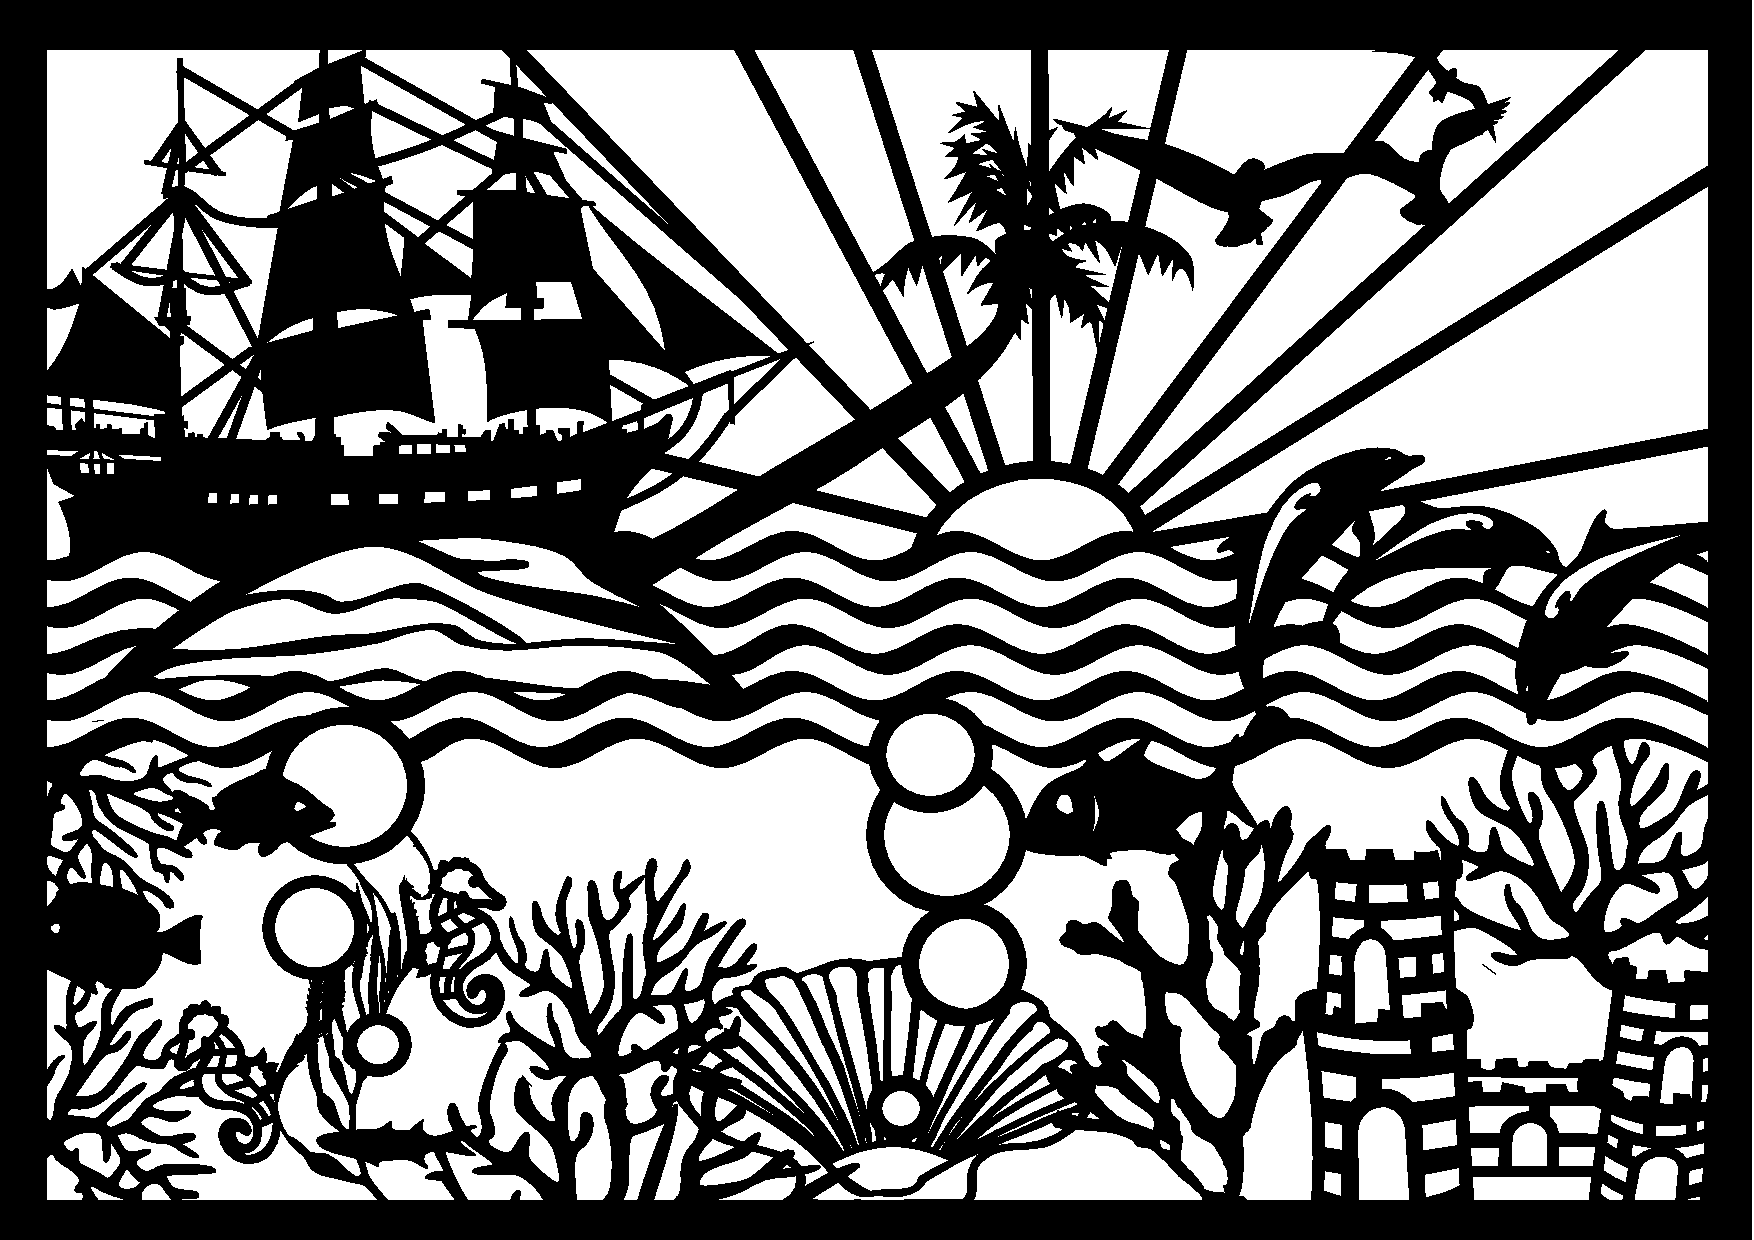
\includegraphics
       [width=3cm]{ozean}
ist ein Bild.
\end{LTXexample}

\noindent Wird das Paket \texttt{graphicx} mit der Option \texttt{[draft]} geladen,
dann erscheint anstelle des Bildes nur ein Rahmen entsprechend
der tatsächlichen Bildgröße mit dem Namen des Grafikfiles, 
was die Bearbeitung beschleunigt und für Probeausdrucke nützlich ist.

Weitere Informationen zum Einbinden von Bildern finden Sie in der
Online"=Dokumentation \cite{grfguide}, im \textit{Graphics Companion}
\cite{grfcomp} und in K.~Reckdahls empfehlenswertem  Tutorium \cite{epslatex}.




%: Seitenaufbau
%!TEX root = l2kurz-Tutorium.tex

% master: l2kurz.tex


\section{Seitenaufbau}

\subsection{Kopf- und Fußzeilen} 
Der Inhalt von Kopf- und  Fußzeilen kann mit dem Befehl
\begin{beispiel}
\lstinline|\pagestyle{|\textit{style}\lstinline|}|
\end{beispiel}
festgelegt werden:
 
Mit \lstinline|\pagestyle{plain}| steht
die Seitennummer zentriert in der Fußzeile; 
das ist die Voreinstellung und braucht normalerweise nicht explizit 
angegeben zu werden.
Mit dem Stil \texttt{headings} stehen Kapitel-Überschrift und
Seitennummer in der Kopfzeile.
Mit \texttt{empty} sind Kopf- und Fußzeile leer.  Der Befehl
\begin{beispiel}
\lstinline|\thispagestyle{|\textit{style}\lstinline|}|
\end{beispiel}
gilt entsprechend nur für die aktuelle Seite.  Einige Befehle, wie etwa
\lstinline|\chapter|, ändern den Stil der aktuellen Seite.  Diese Änderungen 
kann man durch einen nachfolgenden \lstinline|\thispagestyle|-Befehl aufheben.

Im \manual\ ist angegeben, wie man das Aussehen der Kopf- und Fußzeilen
außerdem mit dem Seitenstil 
\lstinline|myheadings| und den Befehlen
\lstinline|\markboth|,
\lstinline|\markright| und
\lstinline|\pagenumbering|
beeinflussen kann. Zur Gestaltung der Kopf- und Fußzeilen stehen die Pakete \texttt{scrpage2}
oder \texttt{fancyhdr} zur Verfügung, die dem Nutzer die Anpassungen erleichtern.

\subsection{Gleitobjekte} \label{floats}
Große Bilder und lange Tabellen lassen sich nicht immer genau 
dort unterbringen, wo sie inhaltlich hingehören, weil sie nicht mehr 
vollständig auf die aktuelle Seite passen, aber auch nicht durch einen 
Seitenwechsel zerrissen werden sollen.  Um  solche Strukturen automatisch
an eine geeignete Stelle "`gleiten"' zu lassen, kennt \LaTeX{} die beiden 
Umgebungen \texttt{figure} und \texttt{table}.  

\subsubsection{Abbildungen (figure)}
Diese Umgebung ist für die Behandlung von Abbildungen gedacht.
Tatsächlich spielt es aber keine Rolle, \emph{wie} diese erzeugt wurden:
Alles, was zwischen
\lstinline|\begin{figure}| und \lstinline|\end{figure}|
steht, wird automatisch an eine Stelle
gesetzt, wo es komplett hinpasst, ohne durch einen Seitenwechsel
zerrissen zu werden.

Mit \lstinline|\caption{...}| setzt man die Bezeichnung der Abbildung.
Dabei ist nur der Text anzugeben, das Wort "`Abbildung"' und die
fortlaufende Nummer werden von \LaTeX\ hinzugefügt.
Bei Abbildungen ist es allgemein üblich, die Bezeichnung
\emph{unter} das Bild zu setzen.
Mit \lstinline|\label| und \lstinline|\ref| kann man die Nummer der
Abbildung im Text ansprechen, mit \lstinline|\pageref| ihre Seitenzahl.
Der Befehl \lstinline:\label: muss dabei \emph{nach} dem \lstinline:\caption:-Befehl
stehen, sonst stimmt die Nummerierung nicht! Wie bereits in der Einführung zum Inhaltsverzeichnis
erläutert, benötigt \LaTeX{} mindestens zwei Durchläufe für das korrekte setzen der Nummern und
des Verweises.

Im folgenden Beispiel wird einfach mit dem Befehl \lstinline|\vspace|
(siehe Abschnitt \ref{vabstaende})
leerer Raum für ein später einzusetzendes Bild gelassen:%\todo{PG: besseres Beispiel als ein so leerer weißer Fleck?}:

\begin{LTXexample}[preset=\let\label\origlabel]
Abbildung~\ref{weiss} auf
S.~\pageref{weiss} zeigt
ein Beispiel aus der 
Minimal art.
\begin{figure}[!htb]
\centering
\vspace*{1cm}
\caption{Landschaft im
Nebel} \label{weiss}
\end{figure}
\end{LTXexample}


\LaTeX\ kann eine Abbildung nach verschiedenen Kriterien platzieren:
\texttt{h} "`here"' (hier),
\texttt{t} "`top"' (oben auf der Seite), \texttt{b} "`bottom"' (unten
auf der Seite) oder \texttt{p} "`page"' (eigene Seite für
Abbildungen).

Die Parameter in den eckigen Klammern, die wahlweise angegeben
werden können, dienen dazu, die Platzierung der Abbildung auf die
angegebenen Orte \emph{einzuschränken}.  Durch Angabe von
z.\,B.\ \texttt{tb}
wird \LaTeX{} angewiesen, nur eine Platzierung oben oder unten auf der
Seite zu versuchen, je nachdem,
wo \emph{zuerst} eine passende Stelle gefunden wird.
Werden keine Parameter (und keine eckigen
Klammern!) angegeben, ist die Voreinstellung \texttt{tbp},
also ohne~\texttt{h}.

Eine Platzierungsbeschränkung \emph{nur} auf \texttt{[h]} ist unsinnig;
sie würde das "`Gleiten"' ja gerade verhindern.
Wenn der Platz "`hier"' nicht ausreicht, 
verschiebt \LaTeX{} dann die Abbildung mindestens 
bis zum Anfang der nächsten Seite, so als hätte man \texttt{[ht]} angegeben.

Eine Abbildung, die nicht platziert werden konnte, wird von
\LaTeX\ immer weiter nach hinten verschoben (und schiebt alle
weiteren Abbildungen vor sich her!), bis ein neues Kapitel
beginnt, das Dokument zu Ende ist, oder der Befehl
\lstinline|\clearpage| eingegeben wird.  


Es gibt noch einen weiteren Platzierungsparameter, 
\texttt{!} (bang), der \LaTeX{} anweist,
gewisse eingebaute Beschränkungen zu ignorieren, 
z.\,B., dass bei der Platzierung gemäß \texttt{h}, \texttt{t} oder \texttt{b}
ein Mindestanteil der Seite für normalen Text übrig bleiben muss.
"`Bang"' muss immer zusammen mit mindestens einem der vier
anderen Parameter benutzt werden.  
 


\subsubsection{Tabellen (table)}

Damit Tabellen nicht auf einen Seitenwechsel fallen,
können sie, analog zu Abbildungen, zwischen
\lstinline|\begin{table}| und \lstinline|\end{table}| gesetzt werden.
Die Befehle
\lstinline|\caption|, \lstinline|\label|, \lstinline|\ref| und \lstinline|\pageref|
wirken entsprechend.
Hier sind beide möglichen Konventionen verbreitet: Die
Bezeichnung wird entweder immer \emph{über} oder immer
\emph{unter} die Tabelle gesetzt.

Auch hier gilt, dass in der \texttt{table}"=Umgebung  beliebiger
Text stehen darf; die Tabelle muss nicht zwangsläufig durch die
\texttt{tabular}"=Umgebung erzeugt worden sein.
Der Unterschied zu \texttt{figure} besteht nur darin, 
dass die Bezeichnung mit dem Wort "`Tabelle"' versehen wird,
und dass die Tabellen unabhängig von den Abbildungen nummeriert werden.

\endinput

\clearpage
%: Schriften
%!TEX root = l2kurz-Tutorium.tex

% master: l2kurz.tex
% l2k5.tex - 5.Teil der LaTeX2e-Kurzbeschreibung v2.3
% 2001-04-10 (WaS)

\section{Schriften}
Normalerweise wählt \LaTeX\ die Größe und den Stil der Schrift
aufgrund der Befehle aus, die die logische Struktur des Textes angeben:
Überschriften, Fußnoten, Hervorhebungen usw.
Im folgenden werden Befehle und Makropakete beschrieben, mit denen
die Schrift auch explizit beeinflusst werden kann.
Ausführlichere Erläuterungen zum Umgang mit Schriften in \LaTeX{}
findet man im \textit{\LaTeX-Begleiter} \cite{wonne}
und in der Online-Dokumentation \cite{fntguide}.

\subsection{Schriftgrößen}
 
Die in der Tabelle~\ref{sizes} angeführten Befehlen 
wechseln die Schriftgröße.
Sie spezifizieren die Größe relativ
zu der von \lstinline:\documentclass: festgelegten Grundschrift.
Ihr Wirkung reicht bis zum Ende der aktuellen Gruppe oder Umgebung.


\begin{table}[!htb]
\caption{Schriftgrößen} \label{sizes}
\def\arraystretch{1.25}
\centering
\begin{tabular}{@{}ll@{}}
\toprule
\lstinline|\tiny|         & \tiny        winzig kleine Schrift \\
\lstinline|\scriptsize|   & \scriptsize  sehr kleine Schrift (wie Indizes)\\
\lstinline|\footnotesize| & \footnotesize     kleine Schrift (wie Fußnoten)\\
\lstinline|\small|        & \small            kleine Schrift \\
\lstinline|\normalsize|   & \normalsize  normale Schrift \\
\lstinline|\large|        & \large       große Schrift \\
\lstinline|\Large|        & \Large       größere Schrift \\
\lstinline|\LARGE|        & \LARGE       sehr große Schrift \\[3pt]
\lstinline|\huge|         & \huge        riesig groß \\[3pt]
\lstinline|\Huge|        & \Huge        gigantisch \\
\bottomrule
\end{tabular}
\end{table}
 
Die Größen-Befehle verändern auch die Zeilenabstände auf
die jeweils passenden Werte -- aber nur, wenn die
Leerzeile, die den Absatz beendet, innerhalb des
Gültigkeitsbereichs des Größen-Befehls liegt:

\begin{LTXexample}
{\Large zu enger \\
Abstand}\par
\end{LTXexample}

\begin{LTXexample}
{\Large richtiger\\
Abstand\par}
\end{LTXexample}

Für korrekte Zeilenabstände darf die
schließende geschwungene Klammer also nicht zu früh kommen,
sondern erst nach einem Absatzende, das übrigens nicht nur als
Leerzeile, sondern auch als Befehl \lstinline|\par|  eingegeben werden 
kann.


\subsection{Schriftstil}
Der Schriftstil wird in \LaTeX{} durch 3~Merkmale definiert:
\begin{description}
\item[Familie] Standardmäßig stehen 3~Familien zur Wahl:
  "`roman"' (Antiqua), "`sans serif"' (Serifenlose) und "`typewriter"'
  (Schreibmaschinenschrift).
\item[Serie] Die Serie gibt Stärke und Laufweite der
  Schrift an: "`medium"' (normale Schrift), "`boldface extended"'
  (fett und breiter).
\item[Form] Die Form der Buchstaben: "`upright"'
  (aufrecht), "`slanted"' (geneigt), "`italic"' (kursiv),
  "`caps and small caps"' (Kapitälchen).
\end{description}
Tabelle~\ref{fonts} zeigt die Befehle, mit denen diese Attribute 
explizit beeinflusst werden können.  
Die Befehle der Form \lstinline|\text...| setzen nur ihr Argument im 
gewünschten  Stil.  Zu jedem dieser Befehle ist ein Gegenstück angegeben, 
das von seinem Auf\/treten an bis zum Ende der laufenden Gruppe oder Umgebung 
wirkt.

Zu beachten ist, dass Wörter in Schreibmaschinenschrift nicht automatisch
getrennt werden.\par

\begin{table}[hbp]
\caption{Schriftstile} \label{fonts}
\def\arraystretch{1.25}
\centering
\begin{tabular}{@{}lll@{}}
\toprule
\lstinline|\textrm|\{\textit{text}\}     &\lstinline|\rmfamily|   &\textrm{Antiqua}\\
\lstinline|\textsf|\{\textit{text}\}     &\lstinline|\sffamily|   &\textsf{Serifenlose}\\
\lstinline|\texttt|\{\textit{text}\}     &\lstinline|\ttfamily|   &\texttt{Maschinenschrift}\\
\lstinline|\textmd|\{\textit{text}\}     &\lstinline|\mdseries|   &\textmd{normal}\\
\lstinline|\textbf|\{\textit{text}\}     &\lstinline|\bfseries|   &\textbf{fett, breiter laufend}\\
\lstinline|\textup|\{\textit{text}\}     &\lstinline|\upshape|    &\textup{aufrecht}\\
\lstinline|\textsl|\{\textit{text}\}     &\lstinline|\slshape|    &\textsl{geneigt}\\
\lstinline|\textit|\{\textit{text}\}     &\lstinline|\itshape|    &\textit{kursiv}\\
\lstinline|\textsc|\{\textit{text}\}     &\lstinline|\scshape|    &\textsc{Kapitälchen}\\
\lstinline|\textnormal|\{\textit{text}\} &\lstinline|\normalfont| &\textnormal{Die Grundschrift des Dokuments}\\
\bottomrule
\end{tabular}
\end{table}

Die Befehle für Familie, Serie und Form können untereinander und mit den
Größen-Befehlen kombiniert werden;  allerdings muss nicht jede
mögliche Kombination tatsächlich als reale Schrift (Font)
zur Verfügung stehen.

\begin{LTXexample}
{\small Die kleinen \textbf{fetten}
Römer
beherrschten }{\large das
ganze gro"se \textit{Italien}.}
{\Large\sffamily\slshape plakativ}
\end{LTXexample}


Je \emph{weniger} verschiedene Schriftarten man verwendet, desto
lesbarer und schöner wird das Schriftstück!


\subsection{Andere Schriftfamilien}
Mit den im vorigen Abschnitt eingeführten Befehlen kann man nicht beeinflussen,
welche Schriftfamilien tatsächlich als Antiqua, Serifenlose und
Maschinenschrift benutzt werden.  \LaTeX{} verwendet als Voreinstellung
die sog.\ Computer-Modern-Schriftfamilien (CM), siehe Tabelle~\ref{families};
der Stil der mathematischen Zeichensätze passt dabei zu CM~Roman.

Will man andere Schriften benutzen, dann ist der einfachste Weg 
das Laden eines Pakets, das eine oder mehrere dieser Schriftfamilien 
komplett ersetzt.
Tabelle~\ref{families} führt einige derartige Pakete auf%,
% die allerdings nicht in jeder \LaTeX-Installation verfügbar sein müssen
.

Die Dokumentation der \TeX"=Distributionen sollte darüber
informieren, welche Schriften verfügbar sind
und wie Sie weitere installieren und verwenden können.
Insbesondere sollte eine Anzahl von verbreiteten PostScript-Schriften
mit jedem aktuellen \LaTeX-System verwendbar sein \cite{postscript}.


\begin{table}[htb]
\caption[Pakete für alternative Schriftfamilien]
{Pakete für alternative Schriftfamilien \newline\small(Eine leere
Tabellenspalte bedeutet, dass das Paket die betreffende Schriftfamilie nicht 
verändert; * kennzeichnet die jeweils als Grundschrift eingestellte Familie.)}
\label{families}
{\footnotesize
\medskip
\renewcommand{\arraystretch}{1.5}
\newcolumntype{x}{>{\RaggedRight\hspace{0pt}}X}
\begin{tabularx}{\textwidth}{@{}lxxxx@{}}
\toprule
Paket            & Antiqua    & Serifenlose   & Schreibmaschine  & math.\ Formeln\tabularnewline\midrule
(keines)         & CM Roman * & CM Sans Serif & CM Typewriter    & $\approx$ CM Roman\tabularnewline
% \texttt{ccfonts} & Concrete *
%                  &
%                  &
%                  & $\approx$ Concrete\\
% \texttt{cmbright}&
%                  & CM Bright *
%                  & {\raggedright CM\ Typewriter\\ Light}
%                  & $\approx$ CM Bright\\
\texttt{courier} &
                 &
                 & Courier 
                 & \tabularnewline
\texttt{droid}   & Droid Serif~*  & Droid Sans    & Droid Sans Mono &                  \tabularnewline
\texttt{fourier} & Utopia Regular~*    &               &                 & Fourier          \tabularnewline
\texttt{helvet}  & 
                 & Helvetica
                 &
                 & \tabularnewline
\texttt{inconsolata} &                 &                & Inconsolata    &                  \tabularnewline
\texttt{libertine} & Linux Libertine~* & Linux Biolinum &                &                  \tabularnewline
\texttt{lmodern} & LM Roman *          & LM Sans Serif & LM Typewriter & $\approx$ LM Roman \tabularnewline
\texttt{mathptmx}& Times *
                 &
                 &
                 & $\approx$ Times\tabularnewline
\texttt{mathpazo}& Palatino *
                 &
                 &
                 & $\approx$ Palatino\tabularnewline
\bottomrule                
\end{tabularx}
}
\end{table}


\subsection{Die "`europäischen"' Zeichensätze}
\LaTeX{} verwendet standardmäßig  Schriften mit einem Umfang von
128~Zeichen.  Umlaute oder akzentuierte Buchstaben sind darin nicht
enthalten; sie werden jeweils aus dem Grundsymbol und dem Akzent
zusammengesetzt.  

Inzwischen stehen die meisten der mit \LaTeX\ verwendbaren Schriften
auch mit einem erweiterten "`europäischen"' Zeichenvorrat bereit.
Sie enthalten jetzt 256 Zeichen, welche fast
alle europäischen Sprachen abdecken, d.\,h., jedes benötigte
Zeichen ist vorgefertigt in ihnen enthalten.
Das hat nicht nur eine
höhere typographische Qualität zur Folge; aufgrund der inneren Arbeitsweise
von \TeX{} entfallen damit auch die Einschränkungen im Zusammenhang mit
der Silbentrennung, die im Abschnitt~\ref{silb} erwähnt wurden:
Wörter mit Umlauten werden nun besser getrennt, und im Argument des
Befehls \lstinline|\hyphenation| dürfen auch Umlaute und das scharfe~s stehen.

%% stimmt nur fuer EC
%Weiterhin sind die Unterschneidungen im Vergleich zu den amerikanischen
%\TeX-Originalschriften stark verbessert und nun auch auf häufige
%Buchstabenpaarungen in nicht-englischen Sprachen optimiert.

% <------- Formulierung ????
Die europäischen Schriften bestehen aus zwei Teilen: Der T1-Zeichensatz
enthält Buchstaben, ASCII-Zeichen sowie verschiedene Anführungszeichen
und Striche, 
während ein ergänzender TS1-Zeichensatz zusätzliche Textsymbole bereitstellt.
% <------- Formulierung ????

\LaTeX{} wird veranlasst, T1-Schriften zu verwenden,
indem man das Paket \texttt{fontenc} mit der Option \texttt{T1} lädt:
\begin{quote}
  \lstinline|\usepackage[T1]{fontenc}|
\end{quote}
Das Paket \texttt{textcomp} ermöglicht den Zugriff auf die Textsymbole:
\begin{quote}
  \lstinline|\usepackage{textcomp}|
\end{quote}
Welche zusätzlichen Zeichen mit den T1-Schriften
bereitgestellt werden, ist in \cite{usrguide} zusammengefasst;
Anhang~\ref{textsymbols} der vorliegenden Kurzbeschreibung
enthält eine Liste aller TS1-Textsymbole.  Einige der Textsymbole sind
auch ohne das Paket \texttt{textcomp} verfügbar, siehe Abschnitt~\ref{symbole},
dann aber nicht immer in einem zur laufenden Schrift passenden Stil.

Beachten Sie, dass in Fonts, die nicht speziell für die Verwendung 
mit \TeX\ entworfen wurden, 
nur ein Teil der TS1-Textsymbole enthalten ist.
Das betrifft vor allem die "`handelsüblichen"' PostScript-Schriften.

\endinput


\clearpage
%: Umgebungen für Theoreme
%!TEX root = l2kurz-Tutorium.tex

\section{Umgebungen für Theoreme, Definitionen u.\,dgl.}

Im Gegensatz zu anderen Texten folgen mathematische Arbeiten oft einer strengen Gliederung in Definitionen, Theoreme, Lemmata, Beweise, Beispiele, etc.\@ Das Paket \texttt{thmtools} erlaubt das einfache Erstellen von Umgebungen, die diese Gliederung herstellen.
Um das Paket \texttt{thmtools} verwenden zu können ist ein Backend notwendig.
Dazu wird das Paket \texttt{amsthm} geladen (siehe \cite{amsthm}).


Die Definition dieser Umgebungen folgt einem einfachen Schema, dass wir uns im Listing~\ref{thm environments} genauer ansehen.

\begin{figure*}
\begin{example}[caption={Beispiel für die Definition von Theoremumgebungen},
label={thm environments}]
\usepackage{amsthm} % Immer zuerst!
\usepackage{thmtools}

\declaretheorem[
    name=Theorem,
    numberwithin=section
    ]{thm}
	
\declaretheorem[
    name=Lemma,
    numberwithin=section
    ]{lem0}
\end{example}
\end{figure*}

Die erste Definition implementiert eine Umgebung für Theoreme, sie wird mit \cs{begin\{thm\}} geöffnet (Das ist der Ausdruck in den geschwungenen Klammern.).
Weiters wird festgelegt, dass die Umgebung "`Theorem"' heißt und ihre Nummerierung am Anfang jedes Abschnittes zurückgesetzt wird.
Genau so definiert man eine Umgebung für Lemmata (\texttt{lem}). Sehen wir uns ein Beispiel an.

\begin{LTXexample}[firstline=3]
\setcounter{thm}{0}
\setcounter{lem0}{0}
\begin{lem0}
    Sei $n \in \mathbb Z$ 
    beliebig, dann ist $n^2$ 
    genau dann gerade, 
    falls $n$ gerade ist.
\end{lem0}

\begin{thm}
    Die Wurzel aus $2$ ist 
    irrational.
\end{thm}
\end{LTXexample}

Einen kleinen Schönheitsfehler hat diese Konstruktion allerdings: Die Lemmata und Theoreme sollten gemeinsam nummeriert werden. Zu diesem Zweck stellt der Befehl \cs{declaretheorem} die Option \texttt{sibling} zur Verfügung.
Wir definieren die Umgebung für Lemmata mit dieser Option neu:

\begin{example}
\declaretheorem[
    name=Lemma,
    sibling=thm,
    ]{lem}
\end{example}

Im obigen Beispiel erhält man nun den folgenden Output.

\begin{LTXexample}[firstline=2]
\setcounter{thm}{0}
\begin{lem}
    Sei $n \in \mathbb Z$ 
    beliebig, dann ist $n^2$ 
    genau dann gerade, 
    falls $n$ gerade ist.
\end{lem}

\begin{thm}
    Die Wurzel aus $2$ ist 
    irrational.
\end{thm}
\end{LTXexample}

Möchte man ganz auf die Nummerierung verzichten, setzt man die Option \verb|numbered = no|.
Im Paket \texttt{amsthm} ist automatisch eine Umgebung für Beweise namens \texttt{proof} integriert, sodass wir das Lemma einfach beweisen können.
Die Umgebung wird automatisch mit einem Beweisendezeichen ($\square$) beendet.
Weitere Details zu dieser Umgebung finden sich in \cite{amsthm}.

\begin{LTXexample}[firstline=3]
\setcounter{thm}{0}
\setcounter{lem0}{0}
\begin{lem0}
    Sei $n \in \mathbb Z$ 
    beliebig, dann ist $n^2$ 
    genau dann gerade,
    falls $n$ gerade ist.
\end{lem0}

\begin{proof}
    Wenn $n$ gerade ist, 
    so existiert eine 
    weitere ganze Zahl $k$,
    sodass $n = 2 k$ gilt. 
    Durch Quadrieren erhält 
    man $n^2 = 4 k^2$ und 
    $n^2$ ist gerade.
    
    Ist andererseits $n$ 
    ungerade, so gibt es ein 
    $k \in \mathbb Z$, sodass 
    $n = 2 k + 1$ gilt. 
    Es folgt die Identität 
    \[n^2 = 4 k (k + 1) + 1\] 
    und $n^2$ ist ungerade.
\end{proof}
\end{LTXexample}


Der Text innerhalb der Umgebungen, die wir mit \cs{declaretheorem} definiert haben, \emph{kursiv} gesetzt wird. Dies ist für Theoreme und verwandte mathematische Aussagen üblich, nicht jedoch für Definitionen, Bemerkungen oder Beispiele.
Das Paket \texttt{thmtools} stellt zwei vordefinierte Stile -- \texttt{definition} und \texttt{remark} -- zur Verfügung, die den üblichen Stilregeln entsprechen.

\begin{example}
\declaretheorem[
    name=Definition,
    style=definition,
    numbered=no,
    ]{defin}
\end{example}

\begin{LTXexample}
\begin{defin}
    Die Menge der rationalen 
    Zahlen $\mathbb Q$ ist die 
    Menge aller 
    \"Aquivalenzklassen der
    Menge
    \[\lbrace (a, b) \mid 
    a, b \in \mathbb Z, 
    b \neq 0\rbrace\]
    bezüglich der 
    \"Aquivalenzrelation
    \[(a, b) \sim (c, d) 
    :\Leftrightarrow
    ad = cb.
    \]
\end{defin}
\end{LTXexample}

Die Paketdokumentation \cite{thmtools} zu \texttt{thmtools} beschreibt noch viele weitere Anpassungsmöglichkeiten.




\clearpage
%: Literaturverzeichnis
%!TEX root = l2kurz-Tutorium.tex

\section{Literaturangaben}

Mit der \texttt{thebibliography}-Umgebung kann man ein
Literaturverzeichnis erzeugen.
Darin beginnt jede Literaturangabe mit \lstinline|\bibitem|.
Als Parameter wird ein Name vereinbart, unter dem die
Literaturstelle im Text zitiert werden kann, und
dann folgt der Text der Literaturangabe.
Die Nummerierung erfolgt automatisch.
Der Parameter bei \lstinline|\begin{thebibliography}| gibt die
maximale Breite dieser Nummernangabe an, also z.\,B.\
\lstinline|{99}| für maximal zweistellige Nummern.

Im Text zitiert man die Literaturstelle dann mit dem Befehl \lstinline|\cite|
und dem vereinbarten Namen als Argument.

\let\origcite\cite
\begin{LTXexample}[preset=\let\cite\origcite]
Partl~\cite{pa} hat
vorgeschlagen ...

\begin{thebibliography}{99}
\bibitem{pa}
H.~Partl: \textit{German \TeX,}
TUGboat Vol.~9, No.~1 (1988)
\end{thebibliography}
\end{LTXexample}

Werden viele Literatureinträge zitiert bzw. verwendet, bietet sich die Nutzung
einer Datenbank an. Die Datenbank besitzt ihre eigene Syntax,
um die benötigten Literatureinträge zu verwalten. Für die komfortable Verwaltung
von Literaturdatenbanken existieren viele Programme wie beispielsweise JabRef (frei) oder
Endnote (kommerziell). Die Datenbank ist im eigentlichen Sinne eine Textdatei mit
Endung \lstinline|bib|.


Für die Verarbeitung dieser Literaturdatenbanken bieten sich zwei verschiedene
Hilfsmittel für \LaTeX{} an. Die klassische Variante ist \emph{Bib\TeX} in Verbindung
mit einem Literaturverzeichnisstil. Die Anpassung an die eigenen Bedürfnisse
gestaltet sich mehr als schwierig. Daher wurde in den letzten Jahren das \LaTeX{}
Makropaket \emph{biblatex} entwickelt, das alternativ zu \emph{Bib\TeX} das mächtigere
Programm \emph{biber} nutzen kann. Das Makropaket \emph{biblatex} erlaubt die Manipulation
des Literaturverzeichnisses auf \LaTeX"=Ebene. Auf CTAN ist eine deutsche Übersetzung der Dokumenation
verfügbar \cite{biblatex-de}.
\clearpage
%: Spezialitäten
%!TEX root = l2kurz-Tutorium.tex

% master: l2kurz.tex
% l2k6.tex - 6.Teil der LaTeX2e-Kurzbeschreibung v2.3
% 2003-04-10 (WaS)

\section{Spezialitäten}

Das komplette Menü der Spezialitäten, die von \LaTeX\ serviert
werden, ist im \manual\ und in der Online-Dokumentation beschrieben.
Hier soll nur auf einige besondere "`Schmankerln"' hingewiesen
werden.

\subsection{Abstände}

\subsubsection{Zeilenabstand}

Um in einem Schriftstück größere Zeilenabstände zu verwenden,
als es in der Dokumentklasse vorgesehen ist, gibt es in
\LaTeX\ den Befehl \lstinline:\linespread:, der im Vorspann stehen sollte
und dann auf das gesamte Dokument wirkt.  Das kann beispielsweise
dann notwendig werden, wenn eine Schrift benutzt wird, die eine größerer x-Höhe
hat als die voreingestellte Computer-Modern.  Für die Schrift "`Palatino"' etwa
ist eine Vergrößerung des Zeilenabstandes um ca.\ 5\,\% angemessen:
\begin{quote}
\lstinline|\usepackage{mathpazo}|\\
\lstinline|\linespread{1.05}|
\end{quote}

Häufig wird ein anderthalbfacher Zeilenabstand gewünscht, wobei bspw. Fußnoten ausgenommen
sein sollen. Der Befehle \lstinline:\linespread: macht diese Unterscheidung nicht. Zur
Änderung des Zeilenabstandes sollte daher stets auf das Paket \texttt{setspace} zurückgegriffen werden.



\subsubsection{Spezielle horizontale Abstände}\label{abst:horiz}

Die Abstände zwischen Wörtern und Sätzen werden von \LaTeX\
automatisch gesetzt.
Sonstigen horizontalen Abstand kann man mit den Befehlen
\begin{beispiel}
\lstinline|\hspace{|\textit{länge}\lstinline|}|\\
\lstinline|\hspace*{|\textit{länge}\lstinline|}|
\end{beispiel}
einfügen. Wenn der Abstand auch am Beginn oder Ende einer Zeile
erhalten bleiben soll, muss \lstinline|\hspace*| statt \lstinline|\hspace|
geschrieben werden.

Die Längenangabe besteht im einfachsten Fall aus einer Zahl
und einer Einheit.  Die wichtigsten Einheiten sind in
Tabelle~\ref{units} angeführt.
\begin{table}[!htb]
\caption{Einheiten für Längenangaben} \label{units}
\centering
\def\arraystretch{1.25}
\begin{tabular}{@{}ll@{}}
\toprule
\texttt{mm} & Millimeter                               \\
\texttt{cm} & Zentimeter = 10\,mm                            \\
\texttt{in} & inch $= 25.4\,\mathrm{mm} $                 \\
\texttt{pt} & point $ =(1/72.27)\,\mathrm{in}
                        \approx 0.351\,\mathrm{mm}$         \\
\texttt{bp} & big point $ =(1/72)\,\mathrm{in}
                            \approx 0.353\,\mathrm{mm} $     \\
%\texttt{dd} \> Didot-Punkt \( = (1238/1157)\,\mathrm{pt}
%                              \approx 0.376\,\mathrm{mm} \)   \\
% --- wegen unklarer Definition (0.375 ider 0.376mm) besser nicht benutzen!
\texttt{em}  &  Geviert (doppelte Breite einer Ziffer der aktuellen Schrift)\\
\texttt{ex}   & Höhe des Buchstabens x der aktuellen Schrift \\
\bottomrule
\end{tabular}
\end{table}

Die Befehle in Tabelle~\ref{hspace} sind Abkürzungen zum Einfügen
besonderer horizontaler Abstände.

\begin{table}[!htb]
\caption{Befehle für horizontale Abstände} \label{hspace}
\centering
\def\arraystretch{1.25}
\begin{tabular}{@{}ll@{}}
\toprule
\lstinline|\,|       & ein sehr kleiner Abstand (siehe auch Abschnitt~\ref{abstaende})\\
\lstinline|\enspace| & so breit wie eine Ziffer \\
\lstinline|\quad|    & so breit, wie ein Buchstabe hoch ist
                   ("`weißes Quadrat"') \\
\lstinline|\qquad|   & doppelt so breit wie ein \lstinline|\quad| \\
\lstinline|\hfill|   & ein Abstand, der sich von 0 bis \(\infty\)
                   ausdehnen kann. \\
\bottomrule
\end{tabular}
\end{table}

Der Befehl \lstinline|\hfill|  kann dazu dienen, einen vorgegebenen Platz auszufüllen.

\begin{LTXexample}
\raggedright
Schafft mir\hspace{1.5cm}Raum! \\
$\triangleleft$\hfill
$\triangleright$
\end{LTXexample}



\subsubsection{Spezielle vertikale Abstände} \label{vabstaende}

Die Abstände zwischen Absätzen, Kapiteln usw.\ werden von
\LaTeX\ automatisch bestimmt.
In Spezialfällen kann man zusätzlichen Abstand
\emph{zwischen zwei Absätzen} mit dem Befehl
\begin{beispiel}
\lstinline|\vspace{|\textit{länge}\lstinline|}|
\end{beispiel}
bewirken.
Dieser Befehl sollte immer zwischen zwei Leerzeilen angegeben
werden.
Wenn der Abstand auch am Beginn oder Ende einer Seite erhalten
bleiben soll, muss \lstinline|\vspace*| statt \lstinline|\vspace|
geschrieben werden.
Die Befehle in Tabelle~\ref{vspace} sind Abkürzungen für
bestimmte vertikale Abstände.
\begin{table}[!htb]
\caption{Befehle für vertikale Abstände} \label{vspace}
\centering
\def\arraystretch{1.25}
\begin{tabular}{@{}ll@{}}
\toprule
\lstinline|\smallskip| & etwa $\nfrac{1}{4}$ Zeile \\
\lstinline|\medskip|   & etwa $\nfrac{1}{2}$ Zeile \\
\lstinline|\bigskip|   & etwa 1 Zeile \\
\lstinline|\vfill|     & ein Abstand, der sich von 0 bis $\infty$
                     ausdehnen kann\\
\bottomrule
\end{tabular}
\end{table}

Der Befehl \lstinline|\vfill| in Verbindung mit \lstinline|\newpage|
kann dazu dienen, Text an den unteren Rand einer Seite zu setzen
oder vertikal zu zentrieren.  Beispielsweise enthält der Quelltext
für die zweite Seite der vorliegenden Beschreibung:
\clearpage
\begin{example}
\vfill

Dieses Dokument wurde mit \LaTeX{} gesetzt.
...
\newpage
\end{example}


Zusätzlichen Abstand zwischen zwei Zeilen \emph{innerhalb}
eines Absatzes oder einer Tabelle erreicht man mit dem Befehl
\lstinline|\\[|\textit{länge}\lstinline|]|.

\begin{LTXexample}
Albano Cesara \\
Lindenallee 10 \\[1.5ex]
95632 Pestitz
\end{LTXexample}


% \subsection{\LaTeX-Zeichenprogramme}

% \todo[inline]{PG: hier eine kurze Erwähnung von TikZ und anschließend ein Bild, ohne große Erklärung? Hast du ein griffiges Beispiel oder sollen wir auf tex.sx nach einem fragen? Mehr als eine Seite würde ich auf keinen Fall damit verbrauchen, lieber mit einer Aufzählung, welche Vorteile sowas hat (Schriftart/Farben wie im Dokument, Grafik und Quelle sind beieinander, oftmals genauer als Zeichenprogramme, Verbindungen mit dem Text möglich) - aber auch hier Nachteil: Einarbeitung}


\endinput

\clearpage
%: Anhang
%!TEX root = l2kurz-Tutorium.tex

% master: l2kurz.tex
% L2KA.TEX - Anhang der LaTeX-Kurzbeschreibung v2.2
% 2001-06-08 (WaS)

\appendix
%\settocdepth{1}

\enlargethispage*{2.5\baselineskip}

\section[Mit dem Paket \texttt{textcomp} verfügbare Symbole]{Mit dem Paket \texttt{textcomp} verfügbare Symbole\footnote{Schriften, die nicht speziell für die Verwendung mit
\TeX{} entworfen wurden, enthalten normalerweise nur die mit * markierten Zeichen.}}
\label{textsymbols}
{\small
\begin{tabbing}
\quad\quad\=\texttt{Mtextquotestraightdblbase}\hspace{1cm}\=\quad\quad\=\kill
\textquotestraightbase \> \lstinline+\textquotestraightbase+\textsuperscript{*}  \> \textquotestraightdblbase \> \lstinline+\textquotestraightdblbase+\textsuperscript{*} \\
\texttwelveudash \> \lstinline+\texttwelveudash+\textsuperscript{*}  \> \textthreequartersemdash \> \lstinline+\textthreequartersemdash+\textsuperscript{*} \\
\textleftarrow \> \lstinline+\textleftarrow+ \> \textrightarrow \> \lstinline+\textrightarrow+\\
\textblank \> \lstinline+\textblank+ \> \textdollar \> \lstinline+\$+\textsuperscript{*} \\
\textquotesingle \> \lstinline+\textquotesingle+\textsuperscript{*}  \> \textasteriskcentered \> \lstinline+\textasteriskcentered+\textsuperscript{*} \\
\textdblhyphen \> \lstinline+\textdblhyphen+ \> \textfractionsolidus \> \lstinline+\textfractionsolidus+\textsuperscript{*} \\
\textlangle \> \lstinline+\textlangle+ \> \textminus \> \lstinline+\textminus+\textsuperscript{*} \\
\textrangle \> \lstinline+\textrangle+ \> \textmho \> \lstinline+\textmho+\\
\textbigcircle \> \lstinline+\textbigcircle+ \> \textohm \> \lstinline+\textohm+\\
\textlbrackdbl \> \lstinline+\textlbrackdbl+ \> \textrbrackdbl \> \lstinline+\textrbrackdbl+\\
\textuparrow \> \lstinline+\textuparrow+ \> \textdownarrow \> \lstinline+\textdownarrow+\\
\textasciigrave \> \lstinline+\textasciigrave+\textsuperscript{*}  \> \textborn \> \lstinline+\textborn+\\
\textdivorced \> \lstinline+\textdivorced+ \> \textdied \> \lstinline+\textdied+\\
\textleaf \> \lstinline+\textleaf+ \> \textmarried \> \lstinline+\textmarried+\\
\textmusicalnote \> \lstinline+\textmusicalnote+ \> \texttildelow \> \lstinline+\texttildelow+\textsuperscript{*} \\
\textdblhyphenchar \> \lstinline+\textdblhyphenchar+ \> \textasciibreve \> \lstinline+\textasciibreve+\textsuperscript{*} \\
\textasciicaron \> \lstinline+\textasciicaron+\textsuperscript{*}  \> \textacutedbl \> \lstinline+\textacutedbl+\textsuperscript{*} \\
\textgravedbl \> \lstinline+\textgravedbl+\textsuperscript{*}  \> \textdagger \> \lstinline+\dag+\textsuperscript{*} \\
\textdaggerdbl \> \lstinline+\ddag+\textsuperscript{*} \> \textbardbl \> \lstinline+\textbardbl+\textsuperscript{*} \\
\textperthousand \> \lstinline+\textperthousand+\textsuperscript{*} \> \textbullet \> \lstinline+\textbullet+\textsuperscript{*} \\
\textcelsius \> \lstinline+\textcelsius+\textsuperscript{*}  \> \textdollaroldstyle \> \lstinline+\textdollaroldstyle+\\
\textcentoldstyle \> \lstinline+\textcentoldstyle+ \> \textflorin \> \lstinline+\textflorin+\textsuperscript{*} \\
\textcolonmonetary \> \lstinline+\textcolonmonetary+ \> \textwon \> \lstinline+\textwon+\\
\textnaira \> \lstinline+\textnaira+ \> \textguarani \> \lstinline+\textguarani+\\
\textpeso \> \lstinline+\textpeso+ \> \textlira \> \lstinline+\textlira+\\
\textrecipe \> \lstinline+\textrecipe+ \> \textinterrobang \> \lstinline+\textinterrobang+\\
\textinterrobangdown \> \lstinline+\textinterrobangdown+ \> \textdong \> \lstinline+\textdong+\\
\texttrademark \> \lstinline+\texttrademark+\textsuperscript{*} \> \textpertenthousand \> \lstinline+\textpertenthousand+\\
\textpilcrow \> \lstinline+\textpilcrow+ \> \textbaht \> \lstinline+\textbaht+\\
\textnumero \> \lstinline+\textnumero+ \> \textdiscount \> \lstinline+\textdiscount+\\
\textestimated \> \lstinline+\textestimated+ \> \textopenbullet \> \lstinline+\textopenbullet+\\
\textservicemark \> \lstinline+\textservicemark+ \> \textlquill \> \lstinline+\textlquill+\\
\textrquill \> \lstinline+\textrquill+ \> \textcent \> \lstinline+\textcent+\textsuperscript{*} \\
\textsterling \> \lstinline+\pounds+\textsuperscript{*}  \> \textcurrency \> \lstinline+\textcurrency+\textsuperscript{*} \\
\textyen \> \lstinline+\textyen+\textsuperscript{*} \> \textbrokenbar \> \lstinline+\textbrokenbar+\textsuperscript{*} \\
\textsection \> \lstinline+\S+\textsuperscript{*}  \> \textasciidieresis \> \lstinline+\textasciidieresis+\textsuperscript{*} \\
\textcopyright \> \lstinline+\copyright+\textsuperscript{*} \> \textordfeminine \> \lstinline+\textordfeminine+\textsuperscript{*} \\
\textcopyleft \> \lstinline+\textcopyleft+ \> \textlnot \> \lstinline+\textlnot+\textsuperscript{*} \\
\textcircledP \> \lstinline+\textcircledP+ \> \textregistered \> \lstinline+\textregistered+\textsuperscript{*} \\
\textasciimacron \> \lstinline+\textasciimacron+\textsuperscript{*}  \> \textdegree \> \lstinline+\textdegree+\textsuperscript{*} \\
\textpm \> \lstinline+\textpm+\textsuperscript{*} \> \texttwosuperior \> \lstinline+\texttwosuperior+\\
\textthreesuperior \> \lstinline+\textthreesuperior+ \> \textasciiacute \> \lstinline+\textasciiacute+\textsuperscript{*} \\
\textmu \> \lstinline+\textmu+\textsuperscript{*} \> \textparagraph \> \lstinline+\P+\textsuperscript{*} \\
\textperiodcentered \> \lstinline+\textperiodcentered+\textsuperscript{*} \> \textreferencemark \> \lstinline+\textreferencemark+\\
\textonesuperior \> \lstinline+\textonesuperior+ \> \textordmasculine \> \lstinline+\textordmasculine+\textsuperscript{*} \\
\textsurd \> \lstinline+\textsurd+ \> \textonequarter \> \lstinline+\textonequarter+\\
\textonehalf \> \lstinline+\textonehalf+ \> \textthreequarters \> \lstinline+\textthreequarters+\\
\textsf{\texteuro} \> \lstinline+\textsf{\texteuro}+ \> \texttimes \> \lstinline+\texttimes+\textsuperscript{*} \\
\textdiv \> \lstinline+\textdiv+\textsuperscript{*} \\
\end{tabbing}
}

%{\footnotesize\noindent 
%Schriften, die nicht speziell für die Verwendung mit
%\TeX{} entworfen wurden, enthalten normalerweise nur die mit * markierten Zeichen.
%\par}

%!TEX root = l2kurz-Tutorium.tex

% master: l2kurz.tex
% L2KSYM.TEX - Tabellen zum 3.Teil der LaTeX2e-Kurzbeschreibung v2.0, Erlangen 1998
% L2KSYM.TEX - Tabellen zum 3.Teil der LaTeX2e-Kurzbeschreibung Mainz 1994, 1995
% LKSYM.TEX  - Tabellen zum 3.Teil der LaTeX-Kurzbeschreibung Graz-Wien 1987
% last changes: 1999-09-01 WaS

\section{Liste der mathematischen Symbole}  \label{symbols}

In den folgenden Tabellen sind alle Symbole angeführt, die
standardmäßig im mathematischen Modus verwendet werden
können.  Die mit * versehenen Symbole werden
in \LaTeXe\ nur durch das Paket \texttt{latexsym} bereitgestellt. 
Mit den Paketen \texttt{amssymb}, 
\texttt{mathrsfs} oder \texttt{wasysym} stehen weitere Zeichen zur 
Verfügung. Die in einer \TeX-Distribution üblicherweise vorhandene Übersicht {\selectlanguage{USenglish} The Comprehensive \LaTeX{} Symbol List}\cite{symbols} zeigt viele Symbole und wie sie mit \LaTeX{} zu erreichen sind.

% http://detexify.kirelabs.org/classify.html rein?

\begin{table}[hbp]
\caption{Mathematische Akzente}  \label{mathakz}
\begin{symbols}
$\hat a$    \> \lstinline|\hat a|   \> $\dot a$   \> \lstinline|\dot a|   \> $\check a$    \> \lstinline|\check a|    \\ 
$\tilde a$  \> \lstinline|\tilde a| \> $\ddot a$  \> \lstinline|\ddot a|  \> $\breve a$    \> \lstinline|\breve a|    \\
$\vec a$    \> \lstinline|\vec a  | \> $\acute a$ \> \lstinline|\acute a| \> $\mathring a$ \> \lstinline|\mathring a| \\
$\bar a$    \> \lstinline|\bar a|   \> $\grave a$ \> \lstinline|\grave a| \\
\end{symbols}
\end{table}

 
\begin{table}[!htbp]
\caption{Kleine griechische Buchstaben}
\begin{symbols}
$\alpha$   \> \lstinline|\alpha|    \>$\iota $  \> \lstinline|\iota|
  \>$\varrho$  \> \lstinline|\varrho| \\
$\beta$    \> \lstinline|\beta|     \>$\kappa $ \> \lstinline|\kappa|
  \>$\sigma$   \> \lstinline|\sigma| \\
$\gamma$   \> \lstinline|\gamma|    \>$\lambda $\> \lstinline|\lambda|
  \>$\varsigma$\> \lstinline|\varsigma| \\
$\delta$   \> \lstinline|\delta|    \>$\mu $    \> \lstinline|\mu|
  \>$\tau $    \> \lstinline|\tau| \\
$\epsilon$ \> \lstinline|\epsilon|  \>$\nu $    \> \lstinline|\nu|
  \>$\upsilon$ \> \lstinline|\upsilon| \\
$\varepsilon$\> \lstinline|\varepsilon| \>$\xi $\> \lstinline|\xi|
  \>$\phi$     \> \lstinline|\phi| \\
$\zeta$    \> \lstinline|\zeta|     \>$o $      \> \lstinline|o|
  \>$\varphi $ \> \lstinline|\varphi| \\
$\eta$     \> \lstinline|\eta|      \>$\pi $    \> \lstinline|\pi|
  \>$\chi $    \> \lstinline|\chi| \\
$\theta$   \> \lstinline|\theta|    \>$\varpi $ \> \lstinline|\varpi|
  \>$\psi$     \> \lstinline|\psi| \\
$\vartheta$\> \lstinline|\vartheta| \>$\rho $   \> \lstinline|\rho|
  \>$\omega$   \> \lstinline|\omega| \\
\end{symbols}
\end{table}
 
 
\begin{table}[htbp]
\caption{Große griechische Buchstaben}
\begin{symbols}
$\Gamma$ \> \lstinline|\Gamma|  \>$\Xi$     \> \lstinline|\Xi|
  \>$\Phi$   \> \lstinline|\Phi| \\
$\Delta$ \> \lstinline|\Delta|  \>$\Pi$     \> \lstinline|\Pi|
  \>$\Psi$   \> \lstinline|\Psi| \\
$\Theta$ \> \lstinline|\Theta|  \>$\Sigma$  \> \lstinline|\Sigma|
  \>$\Omega$ \> \lstinline|\Omega| \\
$\Lambda$\> \lstinline|\Lambda| \>$\Upsilon$\> \lstinline|\Upsilon| \\
\end{symbols}
\end{table}


\begin{table}[!htbp]
\caption[Verschiedene sonstige Symbole]%
        {Verschiedene sonstige Symbole
         (* benötigt Paket \texttt{latexsym})}
\begin{symbols}
$\aleph $\> \lstinline|\aleph| \>$\prime $\> \lstinline|\prime| \>
$\forall $\> \lstinline|\forall|  \\
$\hbar $\> \lstinline|\hbar| \>$\emptyset $\> \lstinline|\emptyset| \>
$\exists $\> \lstinline|\exists|  \\
$\imath $\> \lstinline|\imath| \>$\nabla $\> \lstinline|\nabla| \>
$\neg $\> \lstinline|\neg|  \\
$\jmath $\> \lstinline|\jmath| \>$\surd $\> \lstinline|\surd| \>
$\flat $\> \lstinline|\flat| \\
$\ell $\> \lstinline|\ell| \>$\top $\> \lstinline|\top| \>
$\natural $\> \lstinline|\natural| \\
$\wp $\> \lstinline|\wp| \>$\bot $\> \lstinline|\bot| \>$\sharp $\> \lstinline|\sharp| \\
$\Re $\> \lstinline|\Re| \>$\Diamond $\> \lstinline|\Diamond|\textsuperscript{*} \>$\clubsuit $\> \lstinline|\clubsuit| \\
$\Im $\> \lstinline|\Im| \>$\Box $\> \lstinline|\Box|\textsuperscript{*} \>$\diamondsuit $\>
\lstinline|\diamondsuit| \\
$\partial $\> \lstinline|\partial| \>$\triangle $\> \lstinline|\triangle| \>
$\heartsuit $\> \lstinline|\heartsuit| \\
$\infty $\> \lstinline|\infty| \>$\angle $\> \lstinline|\angle| \>
$\spadesuit $\> \lstinline|\spadesuit| \\
$\mho $\> \lstinline|\mho|\textsuperscript{*} \\
\end{symbols}
\end{table}


\begin{table}[!htbp]
\caption{"`Große"' Operatoren}
\begin{trivlist}\item
\begin{tabular}{@{}ccl@{\qquad}cll@{\qquad}ccl@{}}
$\sum$     & $\displaystyle \sum$    & \lstinline|\sum|
  & $\bigcap$    & $\displaystyle\bigcap$    & \lstinline|\bigcap|
  & $\bigodot$   & $\displaystyle\bigodot$   & \lstinline|\bigodot| \\[6pt]
$\prod$    & $\displaystyle\prod$    & \lstinline|\prod|
  & $\bigcup$    & $\displaystyle\bigcup$    & \lstinline|\bigcup|
  & $\bigotimes$ & $\displaystyle\bigotimes$ & \lstinline|\bigotimes| \\[6pt]
$\coprod$  & $\displaystyle\coprod$  & \lstinline|\coprod|
  & $\bigsqcup$  & $\displaystyle\bigsqcup$  & \lstinline|\bigsqcup|
  & $\bigoplus$  & $\displaystyle\bigoplus$  & \lstinline|\bigoplus| \\[6pt]
$\int$     & $\displaystyle\int$     & \lstinline|\int|
  & $\bigvee$    & $\displaystyle\bigvee$    & \lstinline|\bigvee|
  & $\biguplus$  & $\displaystyle\biguplus$  & \lstinline|\biguplus| \\[6pt]
$\oint$    & $\displaystyle\oint$    & \lstinline|\oint|
  & $\bigwedge$  & $\displaystyle\bigwedge$  & \lstinline|\bigwedge|
\end{tabular}
\end{trivlist}
\end{table}


\begin{table}[!htbp]
\caption[Binäre Operatoren]{Binäre Operatoren 
  (* benötigt Paket \texttt{latexsym})}
\begin{symbols}
$+$   \> \lstinline|+|   \>$-$    \> \lstinline|-| \> $\div $\> \lstinline|\div| \\
$\pm $\> \lstinline|\pm| \>$\cap $\> \lstinline|\cap| \>$\vee $\> \lstinline|\vee| \\
$\mp $\> \lstinline|\mp| \>$\cup $\> \lstinline|\cup| \>$\wedge $\> \lstinline|\wedge| \\
$\setminus $\> \lstinline|\setminus| \>$\uplus $\> \lstinline|\uplus| \>
$\oplus $\> \lstinline|\oplus| \\
$\cdot $\> \lstinline|\cdot| \>$\sqcap $\> \lstinline|\sqcap| \>
$\ominus $\> \lstinline|\ominus| \\
$\times $\> \lstinline|\times| \>$\sqcup $\> \lstinline|\sqcup| \>
$\otimes $\> \lstinline|\otimes| \\
$\ast $\> \lstinline|\ast| \>$\triangleleft $\> \lstinline|\triangleleft| \>
$\oslash $\> \lstinline|\oslash| \\
$\star $\> \lstinline|\star| \>$\triangleright $\> \lstinline|\triangleright| \>
$\odot $\> \lstinline|\odot| \\
$\diamond $\> \lstinline|\diamond| \>$\lhd $\> \lstinline|\lhd|\textsuperscript{*} \>
$\dagger $\> \lstinline|\dagger| \\
$\circ $\> \lstinline|\circ| \>$\rhd $\> \lstinline|\rhd|\textsuperscript{*} \>
$\ddagger $\> \lstinline|\ddagger| \\
$\bullet $\> \lstinline|\bullet| \>$\unlhd $\> \lstinline|\unlhd|\textsuperscript{*} \>
$\amalg $\> \lstinline|\amalg| \\
$\bigcirc $\> \lstinline|\bigcirc| \> $\unrhd$ \> \lstinline|\unrhd|\textsuperscript{*} \> 
$\wr$ \> \lstinline|\wr| \\
$\bigtriangleup$ \>\lstinline|\bigtriangleup| \>
$\bigtriangledown$ \> \lstinline|\bigtriangledown|\>\\
\end{symbols}
\end{table}


\begin{table}[!htbp]
\caption[Relationen]%
        {Relationen (* benötigt Paket \texttt{latexsym})}
\begin{symbols}
$< $\> \lstinline|<| \>$>$\> \lstinline|>| \>$=$\> \lstinline|=| \\
$\leq $\> \lstinline|\leq| \>$\geq $\> \lstinline|\geq| \>$\equiv $\> \lstinline|\equiv| \\
$\prec $\> \lstinline|\prec| \>$\succ $\> \lstinline|\succ| \>$\sim $\> \lstinline|\sim| \\
$\preceq $\> \lstinline|\preceq| \>$\succeq $\> \lstinline|\succeq| \>
$\simeq $\> \lstinline|\simeq| \\
$\ll $\> \lstinline|\ll| \>$\gg $\> \lstinline|\gg| \>$\asymp $\> \lstinline|\asymp| \\
$\subset $\> \lstinline|\subset| \>$\supset $\> \lstinline|\supset| \>
$\approx $\> \lstinline|\approx| \\
$\subseteq $\> \lstinline|\subseteq| \>$\supseteq $\> \lstinline|\supseteq| \>
$\cong $\> \lstinline|\cong| \\
$\sqsubseteq $\> \lstinline|\sqsubseteq| \>$\sqsupseteq $\> \lstinline|\sqsupseteq| \>
$\bowtie $\> \lstinline|\bowtie| \\
$\sqsubset$ \> \lstinline|sqsubset|\textsuperscript{*}\>
$\sqsupset$ \> \lstinline|sqsupset|\textsuperscript{*}\>
$\Join$\> \lstinline|\Join|\textsuperscript{*} \\
$\in $\> \lstinline|\in| \>$\ni $\> \lstinline|\ni| \>
$\notin$ \> \lstinline|\notin| \\
$\vdash $\> \lstinline|\vdash| \>$\dashv $\> \lstinline|\dashv| \>
$\models $\> \lstinline|\models| \\
$\smile $\> \lstinline|\smile| \>$\mid $\> \lstinline|\mid| \>
$\doteq $\> \lstinline|\doteq| \\
$\frown $\> \lstinline|\frown| \>$\parallel $\> \lstinline|\parallel| \>
$\perp $\> \lstinline|\perp| \\
$:$ \> \lstinline|:| \> $\propto$ \> \lstinline|\propto| \\
\end{symbols}
\end{table}

\begin{table}[!htbp]
\caption{Negierte Relationen}
\begin{symbols}
$\not< $\> \lstinline|\not<| \>$\not> $\> \lstinline|\not>| \>$\not= $\> \lstinline|\not=| \\
$\not\leq $\> \lstinline|\not\leq| \>$\not\geq $\> \lstinline|\not\geq| \>
  $\not\equiv $\> \lstinline|\not\equiv| \\
$\not\prec $\> \lstinline|\not\prec| \>$\not\succ $\> \lstinline|\not\succ| \>
  $\not\sim $\> \lstinline|\not\sim| \\
$\not\preceq $\> \lstinline|\not\preceq| \>$\not\succeq $\> \lstinline|\not\succeq| \>
  $\not\simeq $\> \lstinline|\not\simeq| \\
$\not\subset $\> \lstinline|\not\subset| \>$\not\supset $\> \lstinline|\not\supset| \>
  $\not\approx $\> \lstinline|\not\approx| \\
$\not\subseteq $\> \lstinline|\not\subseteq| \>$\not\supseteq $\>
\lstinline|\not\supseteq| \>
  $\not\cong $\> \lstinline|\not\cong| \\
$\not\sqsubseteq $\> \lstinline|\not\sqsubseteq| \>$\not\sqsupseteq $\>
\lstinline|\not\sqsupseteq| \>
  $\not\asymp $\> \lstinline|\not\asymp| \\
\end{symbols}
\end{table}


\begin{table}[!htbp]
\caption[Pfeile]%
        {Pfeile
         (Vertikale Pfeile werden als Klammerungssymbole behandelt, 
         alle anderen als Relationen.
         * benötigt Paket \texttt{latexsym}.)}
\begin{symbols}
$\leftarrow $\> \lstinline|\leftarrow| \>$\longleftarrow $\>
\lstinline|\longleftarrow| \>
  $\uparrow $\> \lstinline|\uparrow| \\
$\Leftarrow $\> \lstinline|\Leftarrow| \>$\Longleftarrow $\>
\lstinline|\Longleftarrow| \>
  $\Uparrow $\> \lstinline|\Uparrow| \\
$\rightarrow $\> \lstinline|\rightarrow| \>$\longrightarrow $\>
\lstinline|\longrightarrow| \>
  $\downarrow $\> \lstinline|\downarrow| \\
$\Rightarrow $\> \lstinline|\Rightarrow| \>$\Longrightarrow $\>
\lstinline|\Longrightarrow| \>
  $\Downarrow $\> \lstinline|\Downarrow| \\
$\leftrightarrow $\> \lstinline|\leftrightarrow| \>$\longleftrightarrow $\>
\lstinline|\longleft...| \>
  $\updownarrow $\> \lstinline|\updownarrow| \\
$\Leftrightarrow $\> \lstinline|\Leftrightarrow| \>$\Longleftrightarrow $\>
\lstinline|\Longleft...| \>
  $\Updownarrow $\> \lstinline|\Updownarrow| \\
$\mapsto $\> \lstinline|\mapsto| \>$\longmapsto $\> \lstinline|\longmapsto| \>
  $\nearrow $\> \lstinline|\nearrow| \\
$\hookleftarrow $\> \lstinline|\hookleftarrow| \>$\hookrightarrow $\>
\lstinline|\hookrightarrow| \>
  $\searrow $\> \lstinline|\searrow| \\
$\leftharpoonup $\> \lstinline|\leftharpoonup| \>$\rightharpoonup $\>
\lstinline|\rightharpoonup| \>
  $\swarrow $\> \lstinline|\swarrow| \\
$\leftharpoondown $\> \lstinline|\leftharpoondown| \>$\rightharpoondown $\>
\lstinline|\right...| \>
  $\nwarrow $\> \lstinline|\nwarrow| \\
$\rightleftharpoons $\> \lstinline|\rightleftharpoons| \>\>\>
  $\leadsto $\> \lstinline|\leadsto|\textsuperscript{*} \\
\end{symbols}
\end{table}


\begin{table}[!htbp]
  \caption{Klammern}
\begin{tabbing}
 \hspace{7mm}\=\hspace{2.25cm}\= \hspace{7mm}\=\hspace{3.25cm}\=
 \hspace{7mm}\=\hspace{2.25cm}\= \hspace{7mm}\=\hspace{2.25cm}\=\kill
$($       \> \lstinline|(|       \> $)$       \> \lstinline|)| \>
  $\lceil $ \> \lstinline|\lceil|  \> $\rceil $\> \lstinline|\rceil| \\
$\langle $\> \lstinline|\langle| \> $\rangle $\> \lstinline|\rangle| \>
  $\lfloor $\> \lstinline|\lfloor| \> $\rfloor $\> \lstinline|\rfloor| \\
$[$       \> \lstinline|[|       \> $]$      \>  \lstinline|]| \>
  $\{$      \> \lstinline|\{|      \> $\}$     \> \lstinline|\}| \\
%$\lbrack $\> \lstinline|\lbrack| \> $\rbrack $\> \lstinline|\rbrack| \>
%  $\lbrace $\> \lstinline|\lbrace| \> $\rbrace $\> \lstinline|\rbrace| \\
$|$       \> \lstinline.|.       \> $\|$       \> \lstinline.\|. \>
  $\backslash$ \> \lstinline.\backslash. \\
\end{tabbing}
\end{table}

\iffalse % In einer Kurz(!)anleitung unnoetig
\begin{table}[!htbp]
\caption{Synonyme}
\bigskip
Für manche Symbole stehen mehrere verschiedene Befehle zur
Verfügung.
\begin{symbols}
\>\>  $\ne $\> \lstinline|\ne| oder \lstinline|\neq| \> \lstinline|\not=| \\
\>\>  $\le $\> \lstinline|\le| \> \lstinline|\leq| \\
\>\>  $\ge $\> \lstinline|\ge| \> \lstinline|\geq| \\
\>\>  $\{ $\> \lstinline|\{| \> \lstinline|\lbrace| \\
\>\>  $\} $\> \lstinline|\}| \> \lstinline|\rbrace|  \\
\>\>  $\to $\> \lstinline|\to| \> \lstinline|\rightarrow|  \\
\>\>  $\gets $\> \lstinline|\gets| \> \lstinline|\leftarrow|  \\
\>\>  $\owns $\> \lstinline|\owns| \> \lstinline|\ni|  \\
\>\>  $\land $\> \lstinline|\land| \> \lstinline|\wedge|  \\
\>\>  $\lor $\> \lstinline|\lor| \> \lstinline|\vee|  \\
\>\>  $\lnot $\> \lstinline|\lnot| \> \lstinline|\neg|  \\
\>\>  $\vert $\> \lstinline|\vert| \> \lstinline.|.  \\
\>\>  $\Vert $\> \lstinline|\Vert| \> \lstinline.\|.  \\
\end{symbols}
\end{table}
\fi

\iffalse % Wird jetzt bei den Textsymbolen behandelt
\begin{table}[!htbp]
\caption{Nicht-mathematische Symbole}
\bigskip
Die folgenden Symbole sind im Text-Modus verfügbar:
\begin{symbols}
\dag \> \lstinline|\dag|  \>\S \> \lstinline|\S| \>
 \copyright \> \lstinline|\copyright|  \\
\ddag \> \lstinline|\ddag|  \> \P \> \lstinline|\P| \>
 \pounds \> \lstinline|\pounds|  \\
\end{symbols}
\end{table}
\fi

\endinput

\endinput


\clearpage
%: Literaturverzeichnis
\phantomsection
\addcontentsline{toc}{section}{\refname}
\bibliographystyle{unsrtdin}
{\RaggedRight
\bibliography{l2kurz}}

\end{document}
\endinput
